%! Mode:: "TeX:UTF-8"
%! TEX program = xelatex
\PassOptionsToPackage{quiet}{xeCJK}
\documentclass[withoutpreface,bwprint]{cumcmthesis}
\usepackage{etoolbox}
\usepackage{titlesec} %设置标题靠左
\usepackage{listings} %利用此环境插入py代码
\BeforeBeginEnvironment{tabular}{\zihao{-5}}
\usepackage[numbers,sort&compress]{natbib}  % 文献管理宏包
\usepackage[framemethod=TikZ]{mdframed}  % 框架宏包
\usepackage{url}  % 网页链接宏包
\usepackage{pdfpages} %插入附录部分
% 三线表格式
\usepackage{booktabs}
\usepackage{adjustbox}
\usepackage{subcaption}  % 子图宏包
\newcolumntype{C}{>{\centering\arraybackslash}X}
\newcolumntype{R}{>{\raggedleft\arraybackslash}X}
\newcolumntype{L}{>{\raggedright\arraybackslash}X}
\usepackage{amsmath}
\usepackage{booktabs}
\usepackage{geometry}
\usepackage{graphicx}

%代码附录部分
\usepackage{listings}
\usepackage{xcolor} % 可选：用于设置代码颜色

\lstset{ 
    basicstyle=\ttfamily,
    keywordstyle=\color{blue},
    commentstyle=\color{gray},
    stringstyle=\color{red},
    numbers=left,
    numberstyle=\tiny,
    stepnumber=1,
    numbersep=5pt,
    backgroundcolor=\color{white},
    showspaces=false,
    showstringspaces=false,
    showtabs=false,
    tabsize=2,
}

% 调整页面边距
\geometry{
    a4paper,
    left=2cm,
    right=2cm,
    top=2cm,
    bottom=2cm
}


% 定义部分section标题靠左的命令
\newcommand{\leftalignedsection}[1]{%
    \section*{#1}%
    \addcontentsline{toc}{section}{#1}%
}

% 使用titlesec包设置部分section标题靠左
\titleformat{name=\section,numberless}[block]{\raggedright\bfseries\Large}{}{0pt}{}

\usepackage{graphicx}
\usepackage{amsmath}
\usepackage{geometry}
\usepackage{array}
\usepackage{makecell}

%%%%%%%%%%%%%%%%%%%%%%%%%%%%%%%%%%%%%%%%%%%%%%%%%%%%%%%%%%%%%
%% 正文
\begin{document}

% 使用 center 和 minipage 将表格和标题部分组合在一起并居中
\begin{center} % 整个表格和标题区域居中
    \begin{minipage}{0.75\textwidth} % 调整宽度使内容居中

        % 表格部分
        \begin{center}
            \renewcommand\arraystretch{1.5} % 调整行高
            \begin{tabular}{|p{0.25\linewidth}|p{0.25\linewidth}|} % 将每一列的宽度设为页面宽度的0.25，以实现总宽度0.5
                \hline
                \makecell{队伍编号} & \makecell{MCB2400741} \\ \hline
                \makecell{赛道} & \makecell{(A)} \\ \hline
            \end{tabular}
        \end{center}

        % 表格和标题之间的下划线
        \vspace{0.5em} % 调整表格和下划线之间的间距
        \rule{1\linewidth}{0.4pt} % 下划线，宽度为页面宽度的50%，厚度为0.4pt
        
        % 标题部分
        \begin{center}
            {\Large \textbf{台风的分类与预测}} % 论文标题，字号可调节
        \end{center}

    \end{minipage}
\end{center}

\pagenumbering{gobble}  % 隐藏页码

\begin{abstract}

台风具有显著破坏性，因此路径预测和环境变化模型构建至关重要。本团队基于2024年第13号台风贝碧嘉的数据，开发了路径预测模型并分析降水量、风速及台风中心距离的关系。数据处理中使用\textbf{MATLAB}，通过\textbf{拉格朗日插值}和\textbf{多项式模型}填充缺失值，结合\textbf{K-S检验}验证特征与环境因素的分布差异，使用\textbf{K-Means}进行分类，并采用\textbf{随机森林}和\textbf{高斯过程回归}构建动态路径预测模型，分析气象因素对路径的影响。通过\textbf{DTW}和\textbf{RMSE}评估预测路径的准确性，模型在路径预测和降水量分析上表现优异，为台风灾害预警提供重要支持。

\textbf{对于问题一}，本团队在提取台风数据的关键特征后，运用分类评价模型对台风等级进行了系统性分析。首先，基于\textbf{决策树模型}对不同强度的台风样本进行了分类，以挖掘在特定特征组合下的台风分级准则。随后，结合\textbf{支持向量机（SVM）}和\textbf{长短期记忆网络（LSTM）}，进一步提升分类精度，在边界样本的处理上实现优化。最终，模型不仅能够基于输入特征高效判别台风等级，还能对分类性能进行严谨评估，提供夏秋台风的详细区分分析，从而有效评估模型在台风分级任务中的实际表现和泛化能力。

\textbf{对于问题二}，本团队构建了基于\textbf{支持向量回归}（SVR）、\textbf{动态时间规整}（DTW）以及\textbf{卷积神经网络-长短期记忆网络}（CNN-LSTM）的台风路径预测模型，以提升预测的精确性和稳定性。该模型融合了历史台风数据、气象观测数据及海洋参数等多源异构数据，能够综合提取台风路径的时空特征，并通过\textbf{通道注意力机制}增强特定路径特征的权重。在实验中，模型对台风路径的趋势变化具有高一致性，并在动态时间规整距离（DTW）和\textbf{均方根误差}（RMSE）等评价指标上表现出显著优势。

\textbf{对于问题三}，本团队建立了数学模型，分析了2024年9月16日至18日的第13号台风贝碧嘉，定量描述了风速与降水量的关系，并探讨了降水量如何随距离台风中心变化。为增强数据真实感，分析中加入了\textbf{随机噪声}。模型拟合采用了\textbf{幂律}、\textbf{指数}和\textbf{多项式拟合}，风速与降水量进行了幂律拟合，指数衰减模型描述了降水量随台风中心距离的变化。\textbf{残差分析}验证了拟合效果，表明风速与降水量正相关，降水量在台风中心附近达到峰值，随距离增加呈指数衰减趋势。引入气温、气压等因素进一步优化模型，为台风灾害应急管理提供可靠的科学支持。

\vspace{1em}
\keywords{台风路径预测\quad  灾害预警\quad 动态时间规整\quad  支持向量回归\quad 卷积神经网络-长短期记忆网络 \quad \(K\)-\(S\)检验 \quad 多项式拟合 \quad 通道注意力机制 \quad \(K\)-\(Means\)聚类 \quad }

\end{abstract}
%%%%%%%%%%%%%%%%%%%%%%%%%%%%%%%%%%%%%%%%%%%%%%%%%%%%%%%%%%%%% 

\begin{center}
    \tableofcontents  % 目录
\end{center}

\cleardoublepage  % 清除当前页面并开始新的一页
\pagenumbering{arabic}  % 从正文开始页码为 1

%%%%%%%%%%%%%%%%%%%%%%%%%%%%%%%%%%%%%%%%%%%%%%%%%%%%%%%%%%%%%  
\newpage
\section{问题重述}

\subsection{问题背景}
台风是一种复杂的热带气旋现象，其形成与发展涉及气温、气压、季风等多种气象因子，以及科里奥利力、洋流和风场等动力因素。这一过程受到诸多非线性动力学与热力学的影响，尚未完全揭示。台风往往伴随强风和暴雨，严重影响社会稳定与经济发展。为了深入了解2024年7月至9月期间中国发生的台风事件，本研究对夏季与秋季台风的结构与动力学特性进行了多变量分析，以揭示其在不同季节的变化规律。以2024年第13号台风贝碧嘉为案例，利用其9月13日至17日的观测数据，预测未来数日内的台风移动轨迹。通过构建多变量综合预测模型，研究将采用\textbf{动态时间规整}（Dynamic Time Warping, DTW）算法评估模型预测路径与实际路径的匹配程度，以量化预测精度。
此外，台风登陆后，由于海洋能量逐步消退，其风速和降水强度会随台风中心距离递减。本研究将进一步构建台风登陆后风速和降水变化的动态模型，并基于贝碧嘉台风在9月16日至18日的登陆数据，分析其中心风速强度和潜在降水量的变化规律。该模型有助于为受灾地区的风险管理与预警提供科学依据和支持。

\subsection{问题一：台风特征参数的数学描述与分类模型的构建}

为系统分析台风的特征参数，需对强度、等级、最大风速等关键参数进行数学化描述，并结合气温、气压、季风等气象条件，构建台风分类模型。可通过支持向量机（SVM）或决策树等监督学习算法对台风数据进行训练，确定台风类型的判别边界，从而分类2024年7月与9月在中国发生的台风，揭示夏季和秋季台风在生成机制和影响范围上的差异。进一步分析台风路径数据，明确其经过区域，为理解季节变化对台风动力学的影响提供参考。

\subsection{问题二：多因素台风路径预测模型的构建}

台风路径预测涉及多因素的动态耦合作用，如气温、气压、地球自转偏向力和洋流等。为提升预测精度，可通过构建多变量非线性回归或递归神经网络（RNN）时间序列模型，捕捉这些因素对路径的动态影响。以2024年第13号台风贝碧嘉为例，本团队利用深度\textbf{学习模型、支持向量机}等来构建并训练台风预测模型\textsuperscript{\cite{陈睿2018基于深度学习的台风预测关键技术研究}}，通过动态时间规整（DTW）算法评估预测路径与实际路径的匹配度，从而验证模型的鲁棒性和可靠性，为路径预测提供有力支持。

\subsection{问题三：台风登陆后风速与降水量衰减模型的构建}

台风登陆后风速和降水量的衰减特性是研究台风动力学的关键内容。基于流体力学原理和幂律衰减模型，建立风速和降水量的数学关系模型，描述降水量随距台风中心距离增大而递减的趋势。以贝碧嘉台风9月16日至18日的登陆过程为例，预测其途经区域的风力强度和降水总量，并通过残差分析评估模型的拟合度，以提出进一步改进建议，为科学预警和灾害管理提供数据支持。


%%%%%%%%%%%%%%%%%%%%%%%%%%%%%%%%%%%%%%%%%%%%%%%%%%%%%%%%%%%%% 
\newpage
\section{问题分析}

\subsection{问题一}

在问题一中，本团队旨在通过数据分析方法来揭示台风的特征参数（如强度、风速、降水量等）与其路径中的环境因素（如气温、地形、气压变化和海温等）之间的复杂关系，并据此构建一个分类和评估台风特征的数学模型。首先，将收集历史台风数据和相关气象资料（例如海面温度、气压、湿度、地形特征等），并对数据进行清洗与预处理，以修正缺失值和异常值，可通过插值或填补方法来补全数据。接下来，借助探索性数据分析（\textbf{EDA}），使用统计工具（如皮尔逊相关系数）量化各变量间的关系，以识别特征之间的关联性和模式。为简化特征维度，可运用主成分分析（\textbf{PCA}），然后通过机器学习方法（如K均值聚类或层次聚类）构建分类模型，对台风特征进行自动分类和定性分析，并通过交叉验证优化模型的性能。最终，将2024年7月和9月的气象数据输入训练好的模型，分类出对中国可能有影响的台风类别，分析台风途经的省份，并对比夏秋季台风在强度、持续时间和路径上的差异，探索其季节性成因。

\subsection{问题二}

对于问题二，台风路径预测涉及多种物理与环境因素的综合作用。为提高路径预测的准确性，首先需收集多种数据来源的台风信息，包括历史台风路径数据、气象数据（气压、风速等）、海洋学数据（如海表温度和洋流流向）及地球物理参数（如地形特征和地球自转效应）。数据清洗后，将对缺失数据和异常值进行处理，并通过特征工程提取出关键的路径预测特征。接着，应用特征选择方法优化模型的复杂度与泛化能力，构建适合时间序列分析的深度学习模型或支持向量机模型，并训练和优化台风路径预测。最终，我们将使用该模型预测2024年第13号台风贝碧嘉在9月13日至17日的行进路线。为了验证预测效果，利用动态时间规整（\textbf{DTW}）算法比较预测路径与实际路径的相似性，通过该动态对齐方法评估模型的准确性，从而验证其在未来台风预测中的实用性。

\subsection{问题三}

在问题三中，为深入研究台风登陆后风速和降水量的时空变化规律，本团队将利用深度学习方法来捕捉与地形和气象条件相关的空间分布特征。研究流程包含数据收集、预处理和模型构建三大步骤。首先，收集台风相关的历史数据，如风速、降水量、地形高度、气压和湿度等，并对数据进行清洗、归一化和标准化，使不同特征量纲一致，优化模型性能。随后，通过特征工程提取与台风登陆后变化密切相关的时间依赖特征和空间分布特征。训练模型时，将数据划分为训练集和测试集，最终利用模型预测2024年9月16日至18日台风贝碧嘉登陆后的风速和降水量，特别关注风速的空间衰减和降水量的分布特性。预测结果通过均方误差（\textbf{MSE}）和均方根误差（\textbf{RMSE}）进行误差分析，进一步探讨风速和降水量之间的关系，分析模型不足之处并提出改进建议，为台风应急响应和灾害预警提供科学支持。

%%%%%%%%%%%%%%%%%%%%%%%%%%%%%%%%%%%%%%%%%%%%%%%%%%%%%%%%%%%%% 
\newpage
\section{模型假设}

\noindent 为简化问题，本文做出以下假设：

\begin{itemize}
    \item[] \textbullet \hspace{1em} \textbf{台风登陆后结构及动力过程假设：} 假设台风登陆后虽然能量逐渐消失，但其动力过程保持相对稳定，整体结构不会发生突变，使得台风的特征变化趋于平稳。

    \item[] \textbullet \hspace{1em} \textbf{环境因素的独立影响假设：} 假设各关键环境因素（如气温、气压、洋流、风场）对台风路径的影响是相互独立的，且可以通过叠加模型将其共同作用于台风路径预测。

    \item[] \textbullet \hspace{1em} \textbf{台风特征与环境因素的相关性假设：} 假设台风的强度、等级和风速等特征与周围环境因素之间存在统计相关性，并能通过合理的量化来支持模型的相关分析。

    \item[] \textbullet \hspace{1em} \textbf{台风路径与地理地形的影响假设：} 假设台风路径受到海岸线和地形的影响，并将这些地形特征作为模型的独立变量来调整路径预测。

    \item[] \textbullet \hspace{1em} \textbf{短期稳定性假设：} 假设在短时间尺度内（如数小时至一天），台风的生成、路径和强度变化具备稳定性，从而有利于短期路径变化的预测。

    \item[] \textbullet \hspace{1em} \textbf{历史数据代表性假设：} 假设用于建模的历史台风数据具有代表性，能够涵盖未来台风发生的多种情况，因此历史数据中的规律可合理应用于未来台风的分类和路径预测。
\end{itemize}



%%%%%%%%%%%%%%%%%%%%%%%%%%%%%%%%%%%%%%%%%%%%%%%%%%%%%%%%%%%%% 
\section{符号说明}


\begin{table}[h]
\centering
\renewcommand{\arraystretch}{0.6} % 压缩行间距
\small % 缩小字体
\resizebox{0.75\textwidth}{!}{ % 调整表格宽度
\begin{tabular}{>{\centering\arraybackslash}m{1.5cm} >{\centering\arraybackslash}m{5cm} >{\centering\arraybackslash}m{1.5cm}} % 列居中对齐
\toprule
符号 & 说明 & 单位 \\
\midrule
$K$ & 聚类算法 & 个 \\
$P$ & 降水量 & mm \\
$V$ & 风速 & M/s \\
$D$ & 台风距离中心位置 & m \\
$A$ & 峰值降水量 & Mm \\
$\mu$ & 中心位置 & \textbackslash \\
$\sigma$ & 分布的宽度 & \textbackslash \\
$\phi$ & 纬度 & \textbackslash \\
$\lambda$ & 经度 & \textbackslash \\
$\theta$ & 运动方向 & \textbackslash \\
\bottomrule
\end{tabular}%
}
\end{table}



%%%%%%%%%%%%%%%%%%%%%%%%%%%%%%%%%%%%%%%%%%%%%%%%%%%%%%%%%%%%% 

\newpage
\section{模型的建立与求解}

\subsection{问题一：台风特征参数的数学描述与分类模型的构建与求解}

台风属于热带气旋，是与人类生活和生产关系密切的降雨系统。然而，台风容易造成多种灾害，例如：狂风、暴雨、风暴潮等，对人类的生产生活造成了巨大的影响。研究台风的特征参数（如强度、等级、风速等）与环境因素（如气温、气压、季风等）的关系，有助于建立台风的分类评价模型，从而提高台风的预测和预警能力。本团队基于1945年至今的台风数据，旨在通过数据处理、统计分析和聚类算法，建立台风分类模型，并分析夏台风与秋台风的区别。

\subsubsection{数据预处理}


首先，读取\(Excel\)文件并保留原始列标题,然后对数据中的缺失值进行处理：

\setlength{\leftskip}{4em}  % 设置左边距缩进为两格

\begin{itemize}
    \item \textbf{删除关键参数缺失的行：}如气压、台风等级、台风强度等重要指标。

    \item \textbf{插值法填充缺失值：}对于移动方向和移动速度等参数，可根据相邻时刻的数据进行计算和填充。
\end{itemize}

\setlength{\leftskip}{0em}  % 恢复原始左边距设置

\textbf{拉格朗日插值法}

拉格朗日插值法是一种找到插值多项式的方法，该插值多项式通过给定的离散点来近似一个函数。假设我们有\(n+1\)个数据点($x_{0}$,$y_{0}$),($x_{1}$,$y_{1}$),...,($x_{n}$,$y_{n}$),目标是找到一个多项式$P_{(x)}$使得：

\[P_{x_{i}} = y_{i},\forall i = 0,1,2,...,n \]

插值多项式的形式通常表示为：

\[P_{x}=\sum_{i=0}^{n} y_{i}L_{i}(x)\]

其中，$L_{i}(x)$是称为拉格朗日基函数的部分，它的作用是确保多项式在每个节点上的插值值等于原值。

接着，进行基函数的构造。

拉格朗日基函数$L_{i}(x)$的定义为：

\[L_i(x) = \prod_{\substack{j=0 \\ j \neq i}}^n \frac{x - x_j}{x_i - x_j}\]

基函数$L_{i}(x)$具有以下两个重要的性质：

\begin{itemize}
  \setlength{\itemindent}{2em}
  \item 当 \( x = x_{i} \) 时，\( L_{i}(x) = 1 \)
  \item 当 \( x = x_{j} \)，且 \( j \ne i \) 时，\( L_{i}(x) = 0 \)
\end{itemize}


也就是说，基函数$L_{i}(x)$的作用是保证$P_{x}$在插值点$x_{i}$的值为$y_{i}$，并且在其他插值点的值为零。

详细步骤如下：

为了详细描述拉格朗日插值法的步骤，我们假设有n+2个已知插值点($x_{0}$,$y_{0}$),($x_{1}$,$y_{1}$),...,($x_{n}$,$y_{n}$)。步骤如下：

\vspace{1em}
\textbf{第一步：确定插值法}

准备好插值所需的点。假设我们有n+1个数据点($x_{0}$,$y_{0}$),($x_{1}$,$y_{1}$),...,($x_{n}$,$y_{n}$)，其中$x_{i}$是插值点的横坐标，$y_{i}$是相应的函数值。

\vspace{1em}
\textbf{第二步：构造拉格朗日基函数}

对于每一个插值点($x_{i}$,$y_{i}$)，我们需要构造拉格朗日基函数$L_{i}(x)$。基函数的表达式为：

\[L_i(x) = \prod_{\substack{j=0 \\ j \neq i}}^n \frac{x - x_j}{x_i - x_j}\]

对于每一个i$\in${0,1,2,...,n}，进行如下操作：


\begin{itemize}
    \setlength{\itemindent}{2em}
    \item 设$L_{i}(X)$初始值为1。

    \item 遍历所有的点$x_{j}$，其中j$\neq$i

    \item 每次都将因子$L_{i}(X)$乘以因子$\frac{x - x_j}{x_i - x_j}$
\end{itemize}

\vspace{1em}
\textbf{第三步：构造插值多项式$P(X)$}

构造插值多项式的最终目标是将各个基函数乘上对应的函数值并求和：

\[P_{x}=\sum_{i=0}^{n} y_{i}L_{i}(x)\]

\begin{itemize}
    \setlength{\itemindent}{2em}
    \item 对于每个插值点($x_{i}$,$y_{i}$),计算对应的基函数$L_{i}(x)$。

    \item 使用公式将所有的$y_{i}$和基函数相乘：$P_{x}=y_{0}L_{0}(X)+y_{1}L_{1}(X)+...+y_{n}L_{n}(X)$

    \item 多项式$P_{x}$是通过所有的拉格朗日奇函数进行线性组合而得到的。
\end{itemize}

\vspace{1em}
\textbf{第四步：化简插值多项式}

\begin{itemize}
    \setlength{\itemindent}{2em}
    \item 对于每个插值点($x_{i}$,$y_{i}$),计算对应的基函数$L_{i}(x)$。

    \item 使用公式将所有的$y_{i}$和基函数相乘：$P_{x}=y_{0}L_{0}(X)+y_{1}L_{1}(X)+...+y_{n}L_{n}(X)$

\end{itemize}

\textbf{a.移动方向的计算}

对于缺失的移动方向，根据当前和下一时刻的经纬度计算。利用两点的经纬度，计算航向角（方位角）：

\begin{align*}
\Delta \lambda &= \lambda_2 - \lambda_1 \\
 &= \sin(\Delta \lambda) \cdot \cos(\phi_2) \\
 &= \cos(\phi_1) \cdot \sin(\phi_2) - \sin(\phi_1) \cdot \cos(\phi_2) \cdot \cos(\Delta \lambda) \\
 &= \arctan2(y, x) \\
\text{若 } \theta &< 0, \text{ 则 } \theta = \theta + 360^\circ
\end{align*}

其中，$\phi$为纬度，$\lambda$为经度，$\theta$为移动方向。

\textbf{b.移动速度的计算}

利用两时刻的经纬度和时间差值，计算移动速度：
\begin{align*}
d &= R \cdot cc = 2 \arctan \left( \sqrt{a}, \sqrt{1 - a} \right)a \\
 &= \sin^2 \left( \frac{\Delta \phi}{2} \right) + \cos(\phi_1) \cdot \cos(\phi_2) \cdot \sin^2 \left( \frac{\Delta \lambda}{2} \right)v \\
 &= \frac{d}{\Delta t}
\end{align*}

\vspace{1em}
\textbf{数据编码}

对分类变量进行编码，例如：

\begin{itemize}
    \setlength{\itemindent}{2em}
    \item 台风强度：用数值表示不同的强度等级。

    \item 台风等级：同上述方法，用数值表示不同等级。
\end{itemize}

\vspace{1em}
\textbf{异常值处理}

检测并处理异常值，例如：

\begin{itemize}
    \setlength{\itemindent}{2em}
    \item 风速超过110m/s 或 气压低于 800hPa 的值视为异常。

    \item 使用箱线法检测异常值。

    \item 对异常值进行剔除或替换为合理值。
\end{itemize}

\vspace{1em}
\textbf{数据标准化}

为了消除量纲的影响，对数据进行了标准化的处理：

\[
Z = \frac{X-\mu}{\sigma } 
\]

其中，X为原始数据，$\mu$为均值，$\sigma$为标准差

\begin{table}[ht]
    \centering
    \[
    \begin{array}{cc}
    \hline \text{台风等级} & \text{风速数值} \\
    \hline \text{弱热带低压} & \leq 10.8 \, \mathrm{m/s} \\
    \text{热带低压} & 10.8 \, \mathrm{m/s} - 17.1 \, \mathrm{m/s} \\
    \text{热带风暴} & 17.2 \, \mathrm{m/s} - 24.4 \, \mathrm{m/s} \\
    \text{强热带风暴} & 24.5 \, \mathrm{m/s} - 32.6 \, \mathrm{m/s} \\
    \text{台风} & 32.7 \, \mathrm{m/s} - 41.4 \, \mathrm{m/s} \\
    \text{强台风} & 41.5 \, \mathrm{m/s} - 50.0 \, \mathrm{m/s} \\
    \text{超强台风} & \geq 50.1 \, \mathrm{m/s} \\
    \hline
    \end{array}
    \]
    \caption{台风强度等级划分}
    \label{table:typhoon_intensity_levels}
\end{table}


\subsubsection{统计描述}

计算各变量的基本统计量：

\begin{itemize}
    \item 均值（Mean）：$\bar{X} =\frac{1}{n}\sum_{i=1}^{n} X_{i}$

    \item 标准差（Standard Deviation）：$\sigma = \sqrt{\frac{1}{n-1}\sum_{i=1}^{n}(X_{i}-\bar{X})^{2} } $

    \item 最大值、最小值、四分位数、中位数等。
\end{itemize}

\begin{figure}[htbp]
    \centering
    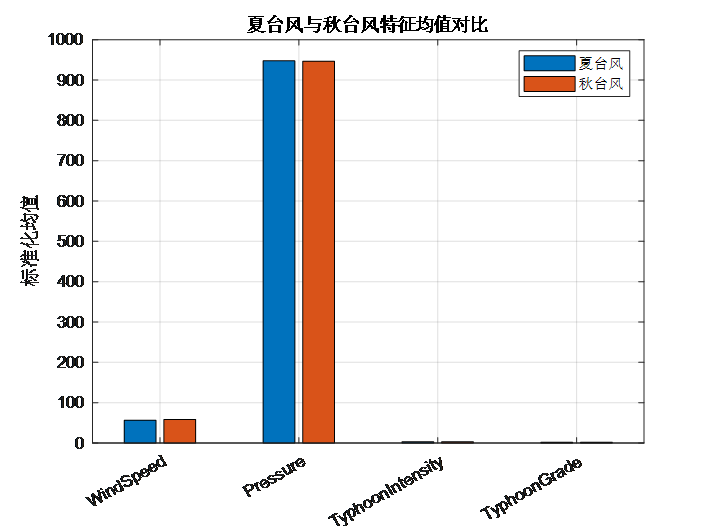
\includegraphics[width=0.75\linewidth]{newFigures/夏秋台风对比.png}
    \caption{夏秋台风对比}
    \label{fig:enter-label}
\end{figure}

\newpage
\textbf{夏秋台风对比如下表所示：}

\begin{table}[h]
\centering
\resizebox{0.75\textwidth}{!}{ % 调整为页面宽度的 0.75
\begin{tabular}{@{}ccc@{}} % 将第一列改为 c 以实现居中
\toprule
特征/台风 & 夏台风 & 秋台风 \\ \midrule
数量 & 15068 & 44645 \\
风速和等级 & 风速高，等级较高 & 风速较低，等级较高 \\
气压特征 & 受低气压条件影响 & 受低气压条件影响 \\
生成位置 & 多生成在低纬度地区 & 高纬度地区 \\
强度 & 较强 & 较弱 \\
路径特点 & 向西北方向移动 & 移动路径没有明显规律 \\ \bottomrule
\end{tabular}
}
\caption{台风特征对比}
\end{table}



\vspace{1em}
\textbf{可能的原因与解释}

\begin{itemize}
    \setlength{\itemindent}{2em}
    \item \textbf{海洋温度}：夏季的高海温为台风提供了大量能量，因此夏台风往往表现出更高的风速和等级。秋季尽管温度下降，但仍然可以维持台风的生成和发展，因此强度没有显著降低。

    \item \textbf{季风效应}：秋季台风受到季风的影响较大，可能导致其移动速度和路径变化更为复杂，这使得它们的风速和等级略低于夏季台风，但强度差异并不显著。

    \item \textbf{气压的相似性}：气压方面，夏秋台风表现相近，可能是因为台风生成时都需要有相对较低的气压中心。无论是夏季还是秋季，台风的低压结构都是驱动其发展的主要因素，因此它们在这一特征上表现出一致性。
\end{itemize}

\vspace{1em}
\textbf{结论}

\begin{itemize}
    \setlength{\itemindent}{2em}
    \item 夏季和秋季台风在风速和等级上存在一定差异，夏台风的风速和等级通常较高。

    \item 气压是台风发展的重要特征，夏台风和秋台风在气压方面表现出很高的相似性，说明两个季节的台风在生成过程中受相似的低压条件影响。

    \item 台风强度在两个季节中的表现差异不大，这表明虽然夏季台风的风速略高，但秋季台风在持续时间和其他强度指标上可能有所弥补，使得整体强度相当。
\end{itemize}

\subsubsection{正态性检验（K-S 检验）}

检验各变量是否服从正态分布，使用Kolmogorov-Smirnov检验：

\begin{itemize}
    \setlength{\itemindent}{2em}
    \item 原假设（$H_{0}$）:数据服从特定分布(正态分布）。

    \item 备择假设（$H_{1}$）:数据不服从特定分布。
\end{itemize}

计算统计量：

\[
D=\sup _{x}\left|F_{n}(x)-F_{0}(x)\right|
\]

其中，$F_{n}(x)$为样本的经验分布函数，$F_{0}(x)$为理论分布函数。


\subsubsection{相关性分析（斯皮尔曼相关系数）}

（1）计算各变量之间的斯皮尔曼相关系数，以分析变量之间的非线性相关性。

（2）使用皮尔逊相关系数进行相关性分析，皮尔逊相关系数也称为皮尔逊积矩相关系数，通常用r表示，是统计学中衡量两个变量线性相关程度的一种指标。其计算公式如下：假设我们有两个变量X和Y，它们各自有一系列观测值$X_{1}$,$X_{2}$,...,$X_{n}$和$Y_{1}$,$Y_{2}$,...,$Y_{n}$。皮尔逊相关系数可以通过以下公式计算得出：

\[
r=\frac{\sum_{i=1}^{n}\left(X_{i}-\bar{X}\right)\left(Y_{i}-\bar{Y}\right)}{\sqrt{\sum_{i=1}^{n}\left(X_{i}-\bar{X}\right)^{2}} \sqrt{\sum_{i=1}^{n}\left(Y_{i}-\bar{Y}\right)^{2}}}
\]

结果如下图所示：

\begin{figure}[htbp]
    \centering
    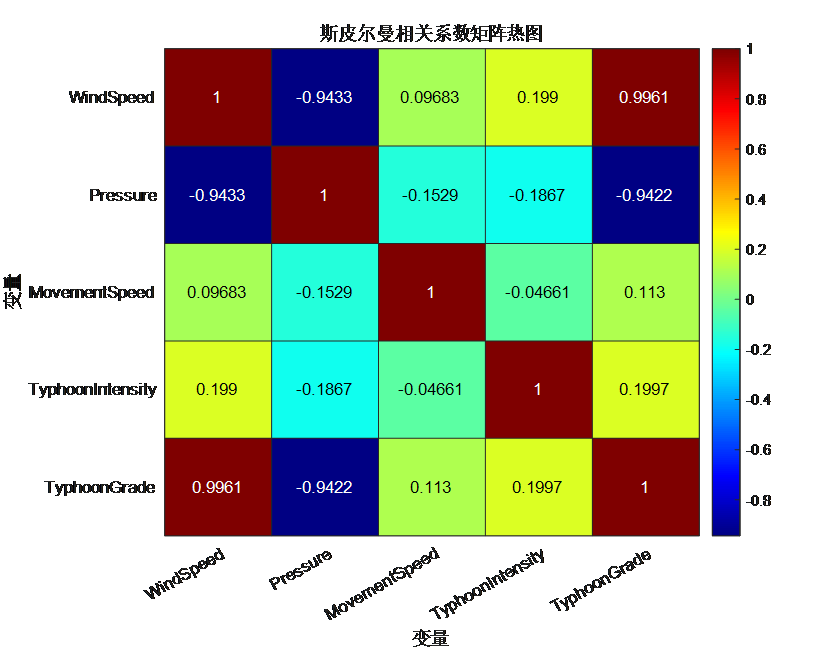
\includegraphics[width=0.75\linewidth]{newFigures/热力图.png}
    \caption{热力图}
    \label{fig:enter-label}
\end{figure}

\begin{itemize}
    \setlength{\itemindent}{2em}
    \item 图的每个单元格代表两个变量之间的\textbf{皮尔逊相关系数}，用不同颜色来表示不同的相关系数值。

    \item \textbf{皮尔逊相关系数}用于衡量两个变量之间的线性关系，取值范围为 -1 到 1。
    
        \begin{itemize}
            \setlength{\itemindent}{2em}
            \renewcommand{\labelitemi}{}  % 取消 itemize 的点
            \renewcommand{\labelitemii}{} % 取消二级项目的标记
            \item +1: 表示两个变量之间存在完全正线性相关关系，即一个变量增大，另一个变量也会同比例增大。
            \item -1: 表示两个变量之间存在完全负线性相关关系，即一个变量增大，另一个变量会同比例减小。
            \item 0: 表示两个变量之间没有线性相关关系。
        \end{itemize}



    \item 热力图中，颜色深浅表示相关系数的大小。通常颜色从深蓝到深红代表从负相关到正相关的程度。
\end{itemize}

\subsubsection{相关性分析}

\textbf{（1）WindSpeed 与其他变量的关系}

\begin{itemize}
    \setlength{\itemindent}{2em}
    \item Pressure（气压）：相关系数为 -0.9433，表示风速和气压之间存在强负相关关系。即当风速增加时，气压通常会降低，反之亦然。这符合台风的物理特性：强烈的风速通常伴随着较低的气压。

    \item MovementSpeed（移动速度）：相关系数为 0.09663，表示风速和移动速度之间的相关性较低，几乎没有明显的线性关系。这表明台风的风速和移动速度并不是直接相关的。

    \item TyphoonIntensity（台风强度）：相关系数为 0.199，表示风速和台风强度之间有较弱的正相关关系。风速的增加可能会导致台风强度略微增加，但这种关系不是特别强。

    \item TyphoonGrade（台风等级）：相关系数为 0.9961，表示风速和台风等级之间几乎存在完全的正相关。这很合理，因为台风的等级通常是根据风速来分类的，风速越大，台风等级越高。
\end{itemize}

\textbf{（2）Pressure 与其他变量的关系}

\begin{itemize}
    \setlength{\itemindent}{2em}
    \item MovementSpeed（移动速度）：相关系数为 -0.1529，表示气压和移动速度之间有弱负相关，关系不显著。这意味着气压变化对台风移动速度的直接影响较小。

    \item TyphoonIntensity（台风强度）：相关系数为 -0.1867，同样表示气压和台风强度之间有较弱的负相关。较低的气压可能意味着更强的台风，但这种影响较小。

    \item TyphoonGrade（台风等级）：相关系数为 -0.9422，表示气压和台风等级之间有很强的负相关。气压越低，台风等级越高，这符合台风的发展机制——气压降低通常意味着台风增强。

\end{itemize}

\textbf{（3）MovementSpeed 与其他变量的关系}

\begin{itemize}
    \setlength{\itemindent}{2em}
    \item TyphoonIntensity（台风强度）：相关系数为 -0.04661，表示移动速度和台风强度之间几乎没有线性相关关系。这表明台风的强度和其移动速度的变化之间不存在显著的线性联系。

    \item TyphoonGrade（台风等级）：相关系数为 0.113，表示移动速度和台风等级之间有非常弱的正相关。这种关系很微弱，可能并不显著

\end{itemize}

\textbf{（4）TyphoonIntensity 与 TyphoonGrade 的关系}

\begin{itemize}
    \setlength{\itemindent}{2em}
    \item TyphoonIntensity 与 TyphoonGrade：相关系数为 0.1997，表示台风强度和台风等级之间有弱正相关关系。台风强度略微影响台风等级，但它不是主要的决定因素，相比之下，风速与等级的相关性更高。

\end{itemize}

\vspace{1em}
\textbf{结论}

\begin{itemize}
    \setlength{\itemindent}{2em}
    \item WindSpeed 和 TyphoonGrade 之间的高度正相关性（0.9961）表明风速是台风等级的主要决定因素，这在台风的分类标准中是合理的，因为台风等级通常是基于风速来定义的。

    \item Pressure（气压）和 WindSpeed（风速）、TyphoonGrade（台风等级）之间的强负相关，意味着气压下降会导致风速和台风等级的增加。这也符合台风形成和发展的基本物理规律。

    \item MovementSpeed（移动速度）与其他变量的相关性普遍较低，表明台风的移动速度与风速、强度、气压等因素之间没有显著的线性关系，这可能是因为台风的移动速度受其他复杂因素（如高空气流、地球自转偏向力等）的影响。

    \item TyphoonIntensity（台风强度）与其他变量之间的相关性普遍不强，说明它不是直接由单一因素决定，而可能是多种因素的共同作用下产生的复杂结果。
    
\end{itemize}

\subsubsection{主成分降维}

主成分分析（PCA）是一种降维方法，将原始变量转化为线性组合的主成分以提取主要信息，并保证主成分之间互不相关、不重叠。PCA通过选取方差最大的变量，将主要注意力集中在变化大的变量上，而变化小的信息则被舍弃，从而减少了维度。通常实际应用中通过样本来估计总体的协方差或相关系数矩阵\textsuperscript{\cite{abdi2010principal}}。设要进行主成分分析的原指标有m个，记为向量x=$x_{1}$,$x_{2}$,$x_{3}$,...,$x_{n}$，现有个样品，相应的观测值为$x_{ik}$(i=1,2,3)，而k = 1,2,3,...,m，记样本协方差矩阵和样本相关系数矩阵分别为:

\[
s_{k}=\frac{1}{n-1}\sum_{i}^{n}(x_{ik}-\bar{x_{k}})(x_{ik}-\bar{x_{k}})^{'}=(s_{ik})      
\]

\[
\hat{R}=(r_{ik}), r_{ik}=\frac{s_{ik}}{\sqrt{s_{ii}}\sqrt{s_{kk}}  }  
\]

其中，$\bar{x_{k}}=\frac{n}{1}\sum_{i=1}{n}x_{ik}$为样本均值。将S作为估计值，$\hat{R}$作为R的估计值，从S或$\bar{R}$出发求样本的主成分。

而当总体各变量的取值的单位或数量级不同时，从总体协方差矩阵出发求解主成分就不合适了，此时需要对每个变量进行标准化变换，将原始变量$x_{k}$标准化为$x_{k}^{*}$，即:

\[
x_{k}^{*} = \frac{x_{k}-\bar{x_{k}}}{s_{k}},k=1,2,3,...,m
\]

其中上述中的$x_{k}^{*}$的平均数为0，标准差为1。

\vspace{1em}
\textbf{主成分分析的一般步骤}

\textbf{a.}将观测数据标准化，并计算$\bar{x_{k}}$及$s_{k}$(k,j=1,2,3,...,m)。

\textbf{b.}有相关系数矩阵R得到的特征值$\lambda_{j}$(j=1,2,3,...m)及各个主成分的方差贡献率、贡献率以及累计贡献率，并根据累计贡献率确定主成分的保留个数p。

\textbf{c.}写出m个基本方程组：

   \[
    \begin{cases}
        r_{11} x_1^{(j)} + r_{12} x_2^{(j)} + \dots + r_{1m} x_m^{(j)} = \lambda_j x_1^{(j)} \\
        r_{21} x_1^{(j)} + r_{22} x_2^{(j)} + \dots + r_{2m} x_m^{(j)} = \lambda_j x_2^{(j)} \\
        \vdots \\
        r_{m1} x_1^{(j)} + r_{m2} x_2^{(j)} + \dots + r_{mm} x_m^{(j)} = \lambda_j x_m^{(j)}
    \end{cases}
    \]
其中，j=1,2,...,m。

利用施密特正交方法，对每一个 $\lambda_j$ 求它的对应基本方程组的解 
    \[
    x_1^{(j)}, x_2^{(j)}, \dots, x_m^{(j)} \quad (j = 1, 2, \dots, m),
    \]
    从而得到用 $\mathbf{x}_1^*, \mathbf{x}_2^*, \dots, \mathbf{x}_m^*$ 表示的
    \[
    b_{kj} = \frac{x_k^{(j)}}{\sqrt{\sum_k \left( x_k^{(j)} \right)^2}}
    \]

    主成分向量 $z_j = \sum_k b_{kj} x_k^*$，或将 $x_k^* = \frac{x_k - \bar{x}_k}{s_k}$ 代入后得到用 $\mathbf{x}_1, \mathbf{x}_2, \dots, \mathbf{x}_m$ 表示的主成分向量
    \[
    z_j = \sum_k b_{kj} x_k^* + a_j
    \]

\textbf{d.} 将 $\mathbf{x}_1, \mathbf{x}_2, \dots, \mathbf{x}_m$ 的观测值代入主成分向量的表达式中计算各个主成分向量。

\textbf{e.} 计算原指标与主成分的相关系数即因子载荷，解释主成分的意义。


\vspace{1em}
\textbf{主成分性质}
\begin{enumerate}
    \setlength{\itemindent}{2em} % 设置缩进量
    \item[a.] 主成分向量的协方差矩阵为对角阵。
    \item[b.] 主成分的总方差等于原始变量的总方差之和。

    设协方差矩阵为 $\sum = (\sigma_{x_i x_k})$，则方差 $D(x_k)$ 为
    \[
    \sum_{k=1}^m D(x_k) = \sum_{k=1}^m \lambda_k = \operatorname{tr}(\sum) = \sum_{k=1}^m \sigma_{kk}
    \]

    由此可见，原始数据的总方差等于个互不相关的主成分的方差之和，说明了个互不相关的主成分包含了原始数据中的所有信息，但是有些主成份所包含有的信息更为集中。

    总方差中的第 $j$ 个主成分 $z_j$ 的方差所占的比例 $\frac{\lambda_j}{\sum_{k=1}^m \lambda_k} (k = 1, 2, \dots, p)$ 称为主成分 $z_j$ 的贡献率。主成分的贡献率反映了主成分综合原始变量信息的能力，也可以理解为解释原始变量的信息能力。由贡献率定义可知，若按照 $m$ 个主成分的贡献率降序排列，则排列之后的各个主成分的综合原始变量信息的能力依次递减。第一个主成分则是贡献率最大的主成分，也即该主成分综合原始变量信息的能力最强，也代表了原始数据中的绝大多数数据信息。

    前 $p (p < m)$ 个主成分的累计贡献率为 $\sum_{j=1}^p \lambda_j = \frac{\sum_{j=1}^p \lambda_j}{\sum_{k=1}^m \lambda_k}$，它反映了前 $p$ 个主成分综合原始变量信息（或解释原始变量）的能力。由于主成分分析的主要目的是降维，所以需要在信息损失不太多的情况下，可以用少数几个主成分来代表原始变量 $\mathbf{x}_1, \mathbf{x}_2, \mathbf{x}_3, \dots, \mathbf{x}_m$，以进行后续的分析。通常以 85\% 为标准，凡是选取的主成分的贡献率之和大于 85\% 即可以达到降维的目的。

    \item[c.] 主成分 $z_{k}$ 与原始变量 $x_{k}$ 之间的相关系数。

    \item[d.] 前 $p$ 个主成分对原始变量 $x_{k}$ 的贡献率。

    \item[e.] 原始变量对主成分 $z_{k}$ 的贡献率。
\end{enumerate}

\subsubsection{台风分类评价模型的建立}

\begin{enumerate}
    \item[(1)] \textbf{选择影响的因素}

    基于相关性分析，选择对台风特征有显著影响的环境因素，如：

        \begin{itemize}
            \item 气温（Temperature）

            \item 气压（Pressure）

            \item 季风（Monson）
        \end{itemize}

    \item[(2)] \textbf{聚类算法的应用}

    采用聚类算法对台风进行分类，常用的聚类算法包括：

        \begin{itemize}
            \item K均值聚类（K-Means Clustering）:

            \begin{itemize}
                \item 确定聚类数K：可以通过肘部法则（Elbow Method）确定最佳K值。

                \item 初始化中心点：随机选择K个初始聚类中心。

                \item 迭代更新：分配样本到最近的聚类中心，o更新聚类中心为当前簇中样本的均值。
            \end{itemize}

            \item 层次聚类（Hierarchical Clustering）

            \begin{itemize}
                \item 计算距离矩阵：计算所有样本之间的距离。

                \item 合并最近的两个簇：根据距离或相似度。

                \item 重复上述步骤，直到所有样本被合并为一个簇。
            \end{itemize}
            
        \end{itemize}

    \item[(3)] \textbf{分类标准的确定}

    根据聚类结果，分析各类别的特征，确定分类标准，例如：

        \begin{itemize}
            \item 强台风：风速大于某一阈值，气压低于某一阈值。

            \item 弱台风：风速和气压均处于较高水平。

        \end{itemize}

        \newpage
        \begin{figure}[htbp]
            \centering
            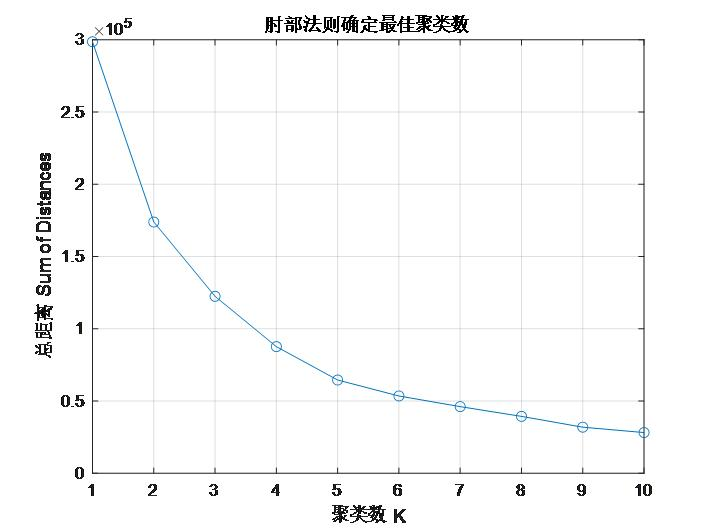
\includegraphics[width=0.75\linewidth]{newFigures/肘部法.jpg}
            \caption{肘部法}
            \label{fig:enter-label}
        \end{figure}

        这幅图显示了聚类数量（K）与总误差平方和（Sum of Squared Distances, SSE）之间的关系。X轴：表示聚类的数量（K），从 1 到 10。Y轴：表示聚类后每个数据点到其所属簇的中心点的总距离的平方和（SSE）。SSE 用于衡量聚类的紧密程度，数值越低表示聚类内部越紧密

\begin{enumerate}
        \item[(a)] 肘部法则的原理：

            肘部法则是一种选择最佳聚类数的方法。它基于在增加聚类数量的情况下，SSE 的变化情况。随着聚类数量的增加，SSE 会减少，因为更多的聚类数意味着簇的尺寸变小，数据点与簇中心之间的距离也相应减少。

            但在某一个聚类数之后，SSE 的减少趋于平缓，曲线变得逐渐平直。这个拐点就被称为“肘部点”，它是选择最佳聚类数的依据。

        \item[(b)] 肘部法则的应用：

             在图中可以看到，SSE 随着 K 的增加不断减少，但在 K = 3 之后，SSE 的减少变得缓慢，曲线开始逐渐趋于平稳。这表明在 K = 3 时，聚类效果和紧密度的提升开始变得不显著。 因此，最佳聚类数量为 3，这个数量可以确保聚类结果既具有合理的紧密性，同时也不会导致过多的类（过度拟合）。
             

        \item[(c)] 肘部位置的选择：

            在图中，肘部位置位于 K = 3，这个点之后，SSE 的下降幅度明显减小，这意味着再增加聚类数所带来的收益已经不如之前那么大。因此，选择 3 作为聚类数是最为合适的。                      
\end{enumerate}
        
\end{enumerate}

\vspace{1em}
\textbf{台风聚类的结果如下图所示：}

\begin{figure}[htbp]
    \centering
    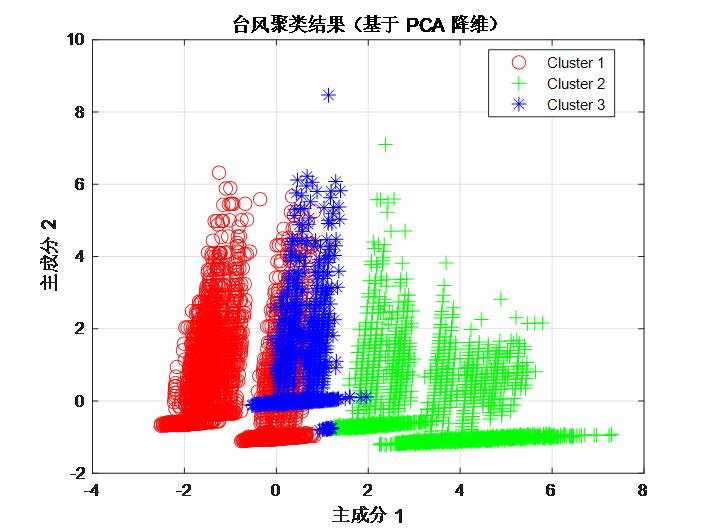
\includegraphics[width=0.75\linewidth]{newFigures/台风聚类的结果.jpg}
    \caption{台风聚类的结果}
    \label{fig:enter-label}
\end{figure}

这幅图显示了通过主成分分析（PCA）降维后的数据在二维空间中的分布，图中用不同颜色和形状的标记代表不同的聚类。

X轴和Y轴分别代表主成分 1和主成分 2，它们是原始数据降维后的两个最主要的方向。

数据在进行聚类之前，通常会使用主成分分析（PCA）进行降维，以便更好地可视化和减少维度之间的冗余信息。在这个图中，使用了两个主成分来表示数据的特征分布，从而在二维空间中显示出不同数据点的聚类情况。

图中显示了三类聚类结果，不同的颜色和形状代表数据被分为不同的类别。


\begin{enumerate}
    \item[(1)]  Cluster 1（红色圆圈）：这一类数据点主要集中在图的左侧和中间靠下的位置。这些点表现出相似的特征，导致它们被分配到同一个类中。

    \item[(2)]  Cluster 2（绿色十字）：这一类主要位于中间偏右和顶部。可以看到这一类的数据点分布比较广泛，涵盖了较大的范围。

    \item[(3)] Cluster 3（蓝色星号）：这一类数据点主要位于中间部分，可以看到它们和 Cluster 1 之间有部分重叠，显示了某种程度的相似性。

\end{enumerate}


聚类分布图显示了在主成分降维后的二维空间中，台风特征样本被划分为三类。Cluster 1 和 Cluster 3 部分重叠，表明二者间边界不甚清晰，可能存在混杂数据点；Cluster 2 的分布较为分散，反映出该类数据在主成分特征上的变异性较大。肘部法则图显示最佳聚类数为 K=3，验证了聚类结果的合理性，且可视化图示了显著的类间差异性。

这两个图表明，通过聚类分析，可以将台风的数据有效地划分为三个主要的类别，不同类别之间具有显著差异，这对于进一步的台风分类研究、路径预测以及影响分析具有重要的参考价值。生成台风路径如下图所示：

\begin{figure}[htbp]
    \centering
    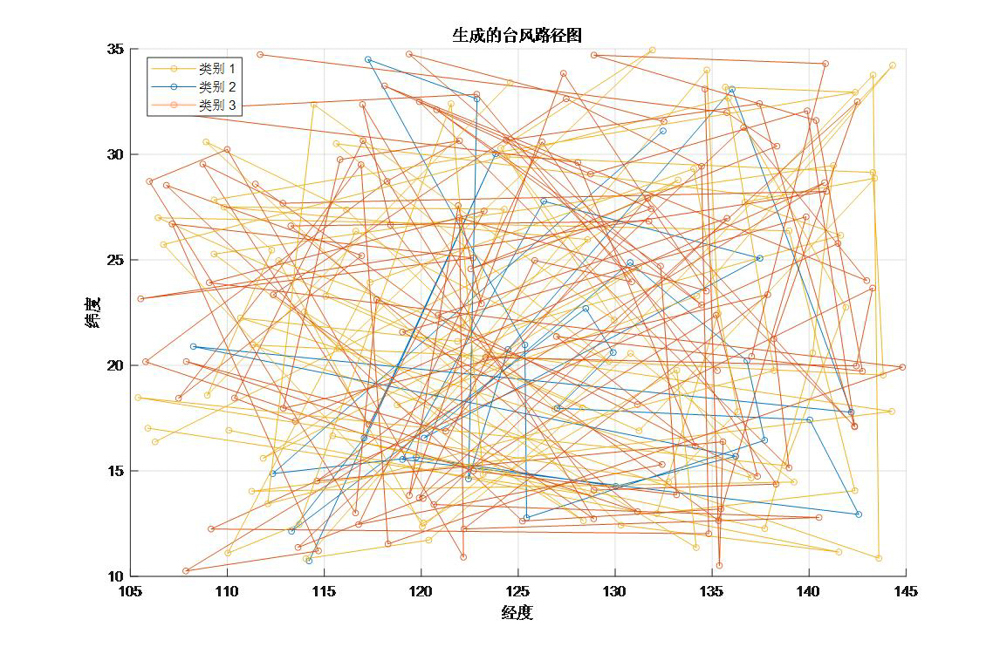
\includegraphics[width=0.75\linewidth]{newFigures/生成台风路径图.jpg}
    \caption{生成台风路径图}
    \label{fig:enter-label}
\end{figure}

\newpage
\subsubsection{模型应用与分析}

\begin{enumerate}
    \item[(1)] \textbf{2024年7月和9月的台风分类}

    利用建立的分类模型，对2024年7月和9月的台风进行分类，得到各台风的类别和途经省份列表。

    \begin{table}[h]
    \centering
    \caption{2024年7月和9月的台风分类}
    \resizebox{0.75\textwidth}{!}{ % 0.75倍页面宽度
    \begin{tabular}{|c|c|c|c|}
    \hline
    月份 & 日期 & 台风类别 & 途经省份 \\ \hline
    \multirow{3}{*}{7月夏台风} 
    & 1980080920 & 2（中等台风） & 福建 \\ \cline{2-4} 
    & 1980082008 & 2（中等台风） & 福建 \\ \cline{2-4} 
    & 1980083002 & 3（弱台风） & 广东 \\ \hline

    \multirow{3}{*}{9月秋台风} 
    & 2018090505 & 1（强台风） & 深圳 \\ \cline{2-4} 
    & 2018091717 & 2（中等台风） & 海南 \\ \cline{2-4} 
    & 2018100105 & 1（强台风） & 福建 \\ \hline
    \end{tabular}
    }
    \end{table}

    \vspace{1em}
    \item[(2)] \textbf{夏台风与秋台风的区别}

    通过比较夏季（6-8月）和秋季（9-11月）台风的特征，分析它们的区别：

\begin{table}[h]
\centering
\resizebox{0.75\textwidth}{!}{ % 调整为页面宽度的 0.75
\begin{tabular}{@{}ccc@{}} % 将第一列改为 c 以实现居中
\toprule
特征 & 夏台风 & 秋台风 \\ \midrule
数量 & 44645 & 15068 \\
风速和等级 & 较高 & 持续时间和强度指标上有所弥补 \\
气压特征 & 高相似性 & 受相似低压条件影响 \\
生成位置 & 多生成于低纬度地区 & 可能生成于较高纬度 \\
强度 & 较强 & 较弱 \\
路径特点 & 向西北方向移动 & 移动路径可能不同 \\ \bottomrule
\end{tabular}
}
\caption{夏台风与秋台风对比}
\end{table}

\end{enumerate}
%%%%%%%%%%%%%%%%%%%%%%%%%%%%%%%%%%%%%%%%%%%%%%%%%%%%%%%%%%%%% 
\newpage
\subsection{问题二：多因素台风路径预测模型的构建与求解}

台风路径预测是一个非常复杂且动态的过程，其受多种物理环境因素的影响，包括台风所处的经纬度位置、大气压力变化、风速、湿度等。台风在海面上的移动受到诸如洋流、气压梯度力、地球自转产生的\textbf{科里奥利力}\textsuperscript{\cite{wie2012development}}等多种复杂力的共同作用。因此，建立一个能够合理模拟这些作用力并综合各种因素影响的数学模型至关重要。台风路径的预测模型需要综合考虑气温、气压、洋流、风场等多重因素，并结合\textbf{动态时间规整算法（Dynamic Time Warping, DTW）}对预测路径与真实路径进行相似性比较。以下步骤概述了模型的构建过程：

\begin{itemize}
    \item 历史台风数据：包括往年台风的位置（如经纬度）、台风强度及其移动速度等。

    \item 气象观测数据：如海面温度(SST)、大气压力、风速和风向等参数，为模型输入提供气候环境因素。

    \item 海洋学观测数据：包含洋流信息，因洋流会对台风路径产生显著影响。

    \item 地球物理参数：主要为地球自转导致的科里奥利力，该力对台风路径有明显偏转作用。
\end{itemize}

\subsubsection{数据预处理}

数据预处理是机器学习建模的关键步骤之一，数据的质量直接影响预测模型的精度。预处理过程包含以下几部分：

\begin{itemize}
    \item \textbf{数据清理：}删除缺失值，去除数据中缺少关键信息（例如经纬度、风速、气压等关键数据）的行，确保模型输入数据的完整性。

    \item \textbf{标准化处理：}为了消除各特征维度差异对模型的潜在干扰，对特征数据进行标准化。标准化公式如下：

                             \[X_{\text {norm }}=\frac{X-\mu}{\sigma}\]

                             其中，$X$ 表示原始特征数据，$\mu$和 $\sigma$分别代表特征的均值和标准差。

    \item \textbf{特征工程：}  选择的特征包括台风的经度 $Lon$、纬度 $Lat$、风速 $WindSpeed$、气压 $Pressure$、移动速度 $MovementSpeed$ 等。我们利用这些特征构建输入矩阵 $X$ 以及目标输出变量 $Y$ 。                  
\end{itemize}

\subsubsection{模型选择}

为有效预测台风路径，本文选择了支持向量回归（Support Vector Regression, SVR）进行建模。选择该方法的原因在于\textbf{SVR}在处理非线性特征方面表现出良好的拟合能力\textsuperscript{\cite{dhiman2019hybrid}}。

\begin{enumerate}
    \item[(1)] 支持向量回归的数学表达式：

                SVR 的目标是寻找一个平滑的函数 $f(x)$，使得模型预测的结果与真实值之间的误差最小。SVR模型的表达式如下：

                \[f(x)=\sum_{i=1}^{n}\left(\alpha_{i}-\alpha_{i}^{*}\right) K\left(x_{i}, x\right)+b\]

                其中：

                \begin{itemize}
                    \item $K(xi,x)$ 为核函数，用于计算样本之间的相似性。通常选择高斯核（RBF 核）来处理复杂的非线性特征。

                    \item  $\alpha_i$ 和 $\alpha_i^*$ 是拉格朗日乘子，通过优化问题求得其具体值。

                    \item $b$ 为偏置项。
                \end{itemize}

    \item [(2)] SVR 的优化目标可以表达为：

                \[\min _{\alpha, \alpha^{*}} \frac{1}{2} \sum_{i=1}^{n} \sum_{j=1}^{n}\left(\alpha_{i}-\alpha_{i}^{*}\right)\left(\alpha_{j}-\alpha_{j}^{*}\right) K\left(x_{i}, x_{j}\right)\]

                在以下约束条件下：

        \begin{itemize}
            \setlength{\itemindent}{2em}
            \renewcommand{\labelitemi}{}  % 取消 itemize 的点
            \item $\begin{array}{c} 0 \leq \alpha_{i}, \alpha_{i}^{*} \leq C \\ \sum_{i=1}^{n}\left(\alpha_{i}-\alpha_{i}^{*}\right)=0 \end{array}$
        \end{itemize}


                其中，其中，$C$ 为惩罚系数，用于控制对预测误差的容忍度。
\end{enumerate}

\subsubsection{模型训练}

\begin{enumerate}
    \item[(1)]定义输入和输出：

              \begin{itemize}
                  \item 输入特征矩阵：我们将主要特征整合为一个矩阵，以便作为模型的输入数据，其中： X = $[\text{Lon}, \text{Lat}, \text{WindSpeed}, \text{Pressure}]$ 

                  \item 输出（目标变量）：为实现台风路径预测，我们将目标变量定义为台风的移动速度，即：Y = $[\text{MovementSpeed}]$
              \end{itemize}

    \item[(2)] 数据分割：

            为了确保模型能够在不同的数据上有效泛化，将数据划分为训练集（占比80\%）和测试集（占比20\%）。通过这种数据划分，模型在测试集上的性能将能更准确反映其对新数据的预测能力。

    \item[(3)]支持向量回归的训练

            利用高斯核函数的支持向量回归模型进行训练。训练的目的是寻找最优的 $\alpha_i$、$\alpha_i^*$ 和偏置项 b ，以便使预测误差达到最小化。
\end{enumerate}

\subsubsection{预测与评估}

\begin{enumerate}
    \item[(1)]预测

                使用已训练的支持向量回归模型( SVR )对测试集进行预测，以生成台风移动速度的预测值。

    \item[(2)]评估指标

                \begin{itemize}
                    \item 均方误差（Mean Squared Error, MSE）：

                             该指标用于衡量预测值与真实值之间的差距。其计算公式为：$\mathrm{MSE} = \frac{1}{n} \sum_{i=1}^{n} (Y_i - \hat{Y}_i)^2v$

                    \item 均方根误差（Root Mean Squared Error, RMSE）

                            \textbf{RMSE} 表示预测值与实际值之间的平均误差\textsuperscript{\cite{willmott2005advantages}}，其计算公式为：$\mathrm{RMSE} = \sqrt{\mathrm{MSE}}$

                             通过 RMSE 可衡量模型预测的精度，其数值越小，表明模型的预测结果与真实值越接近。
                             
                \end{itemize}
\end{enumerate}




\subsubsection{DWT算法的应用}

\begin{enumerate}
    \item[(1)] 动态时间规整（Dynamic Time Warping, DTW）

                \textbf{动态时间规整算法}\textsuperscript{\cite{muller2007dynamic}}是一种用于衡量两条时间序列间相似性的数学方法，尤其适用于时间轴上存在非线性变形的情况。当两个序列的采样点在时间轴上的分布存在非线性拉伸或压缩时，DTW 通过对齐这些点以最小化差异，从而提升匹配精度。

    \item[(2)]  台风路径数据的时序特点

                台风路径数据本质上为时间序列数据，其经纬度随时间演变，且不同时间点的移动速度可能存在较大差异。DTW 可通过匹配不同时刻的路径点，以适应时间序列的动态变化，进而提供两条台风路径的最佳匹配。

    \item [(3)] 距离度量原理

                给定两条时间序列 $A$ 和 $B$，DTW 度量的目的是通过在时间轴上对序列进行拉伸或压缩，来找到二者的最小累积差异路径。应用于台风路径时，DTW 将路径点进行动态对齐，以计算其累积的最短路径距离，距离值越小即代表预测路径与实际台风路径的相似性越高。
                
\end{enumerate}

\subsubsection{台风生命周期及时序特征}

台风的生命周期包括生成、发展、成熟和消亡四个阶段，各阶段的数据随时间发生演化，表现出显著的时间依赖性。台风路径数据每隔6小时采集一次，这种时间连续性保障了数据的完整性，并使台风特征的提取更为精确。

\begin{enumerate}
    \item[(1)] 台风生命周期与时间特征的变化

                在生成阶段，台风能量尚未积聚，风速较低、路径平稳，移动范围也较小。随着台风进入发展和成熟阶段，它会逐步积累能量，风速增强、最低气压降低，导致周围水汽汇聚并增强台风结构，此时台风的移动范围加大，路径曲率增大。最终，在消亡阶段台风能量逐渐衰减，移动路径趋缓直至停止。台风路径的时间依赖性使得上一个阶段的状态对下一阶段起到衔接作用，因此，时间特征的提取是路径预测的核心部分。

    \item[(2)]  长短期记忆神经网络（LSTM）的时序特征提取

                基于循环\textbf{神经网络（RNN）}的\textbf{长短期记忆（LSTM）}神经网络通过增设遗忘门、输入门和输出门三个控制单元，解决了普通神经网络中长序列依赖弱的问题\textsuperscript{\cite{chen2019hybrid}}。LSTM 在读取上下文信息时通过对数据进行筛选保留重要的长时记忆，同时提高模型效率。其提取时间序列特征的具体过程如下：

                \begin{figure}[htbp]
                    \centering
                    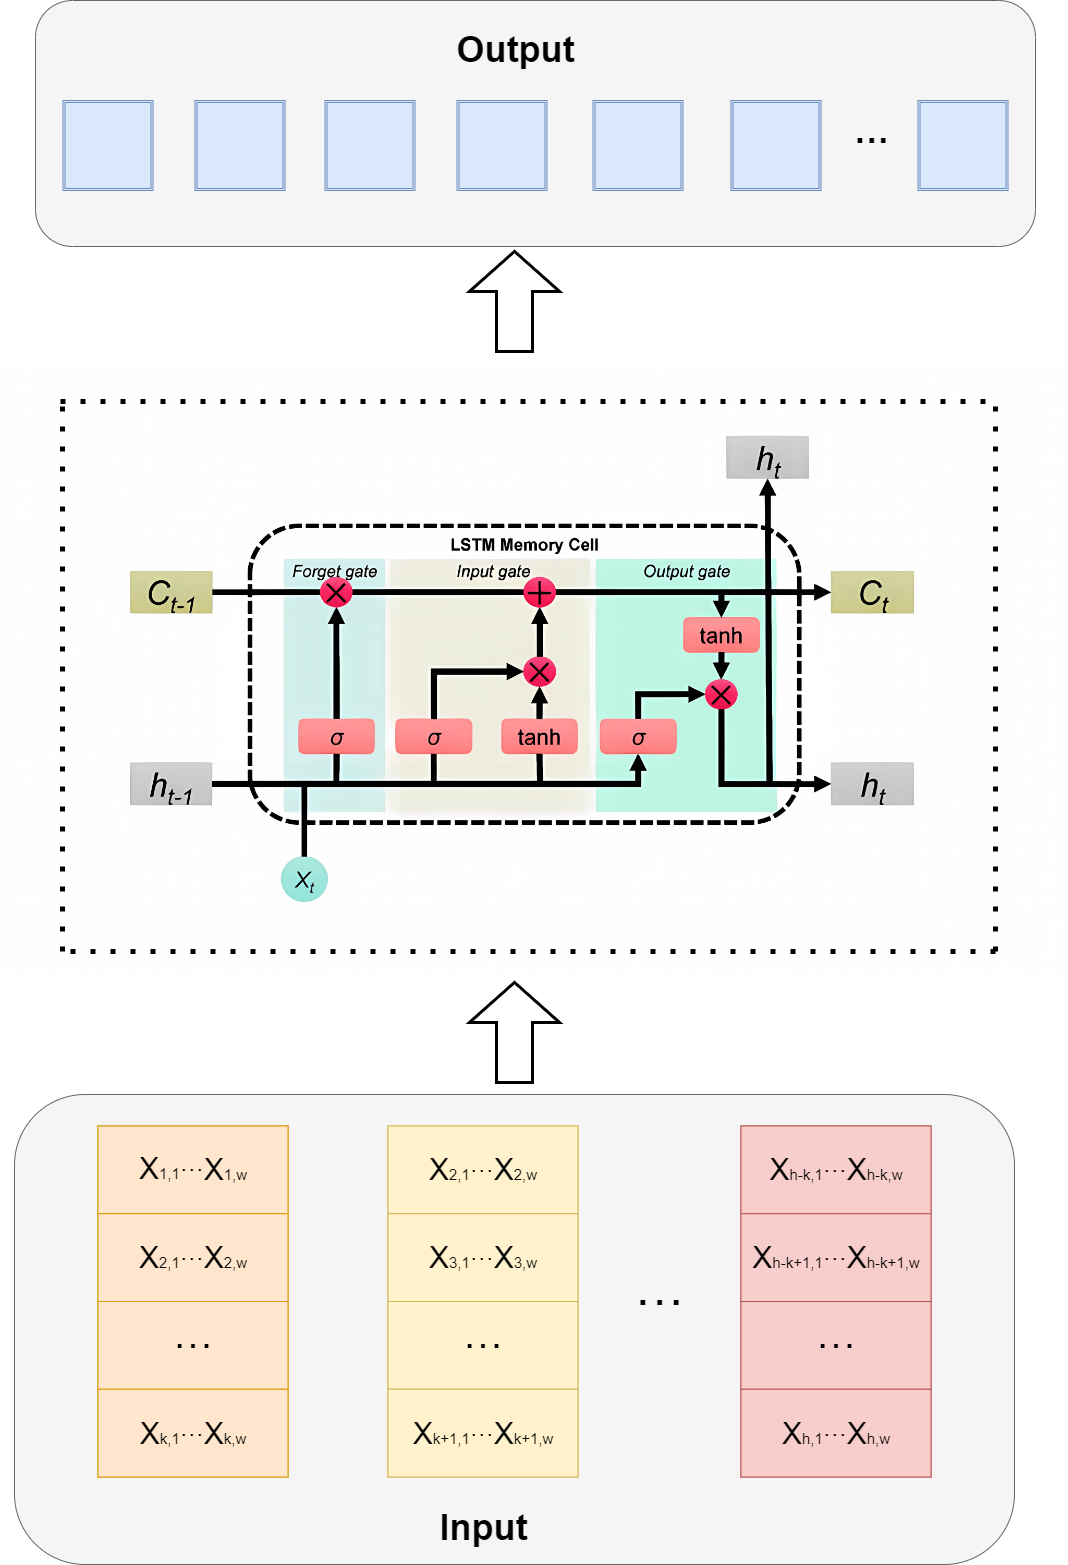
\includegraphics[width=0.5\linewidth]{newFigures/LSTM.png}
                    \caption{LSTM}
                    \label{fig:enter-label}
                \end{figure}
                
\end{enumerate}

\subsubsection{模型结构和多特征融合方法}

在台风路径预测中，路径不仅取决于时间序列数据，还受到空间特征的影响。因此，模型不仅包含\textbf{卷积神经网络（CNN）}来提取空间特征，还引入了\textbf{长短期记忆神经网络（LSTM）}来提取时序特征。

为了有效融合空间和时间特征，本文引入了\textbf{通道注意力机制}\textsuperscript{\cite{he2022dual}}。具体做法是首先将CNN提取的空间特征与LSTM提取的时间特征进行连接，再通过通道注意力机制对这些特征进行动态加权处理，以更集中于路径预测中关键信息。我们采用了“压缩和激励网络”作为注意力机制的实现方法，该网络分为两个部分：

\begin{enumerate}

    \item[(1)]压缩部分：对全局空间信息进行压缩，将数据汇总至通道维度上，以学习各个通道的重要性。

    \item[(2)]激励部分：根据通道重要性分配不同的权重，从而在模型预测过程中对关键特征进行优先处理。

\end{enumerate}

这种注意力机制可以在复杂网络结构下有效增强模型的学习效率，同时确保了网络的拓扑结构不至于过于复杂，以避免学习速度过慢的问题。

\begin{figure}[htbp]
    \centering
    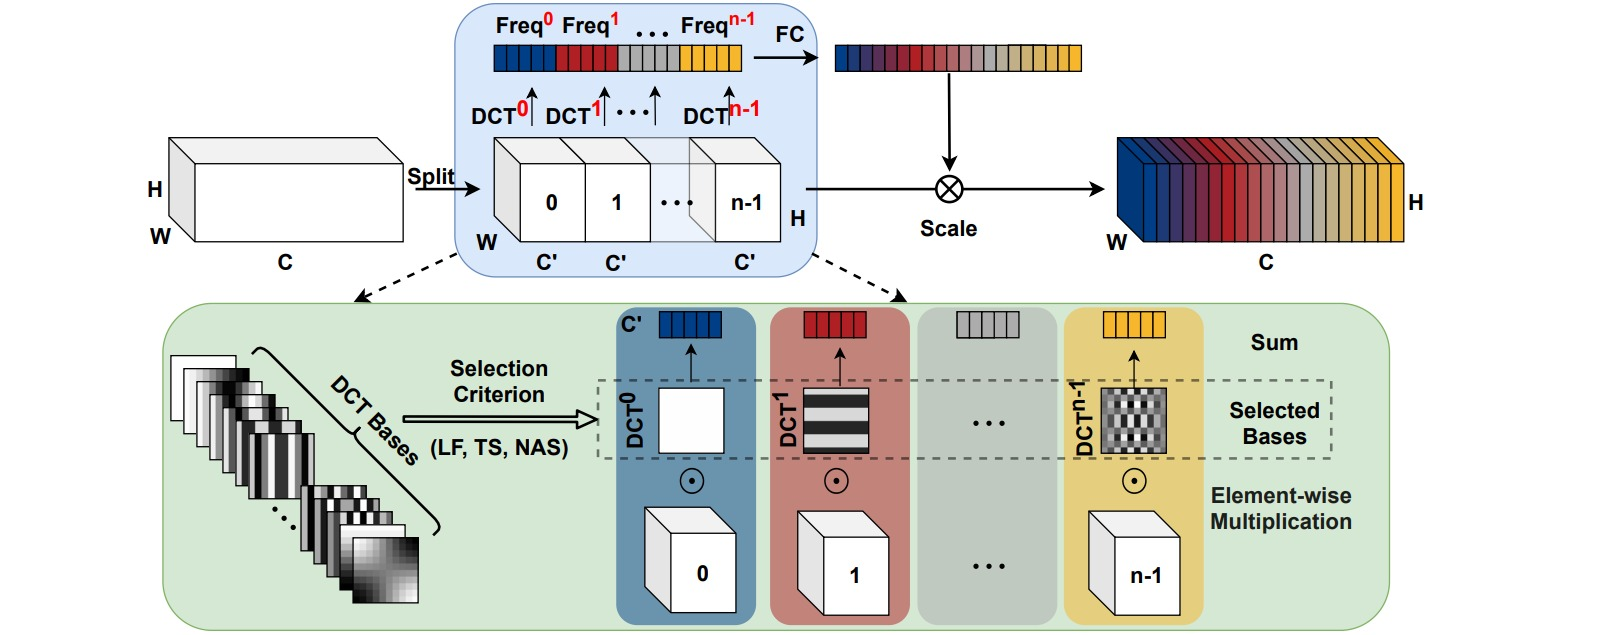
\includegraphics[width=0.75\linewidth]{newFigures/神经网络通道图.jpg}
    \caption{神经网络通道图}
    \label{fig:enter-label}
\end{figure}

\subsubsection{实验结果分析}

\textbf{（1）实际与预测路径的比较（多项式回归模型）}
\begin{figure}[htbp]
    \centering
    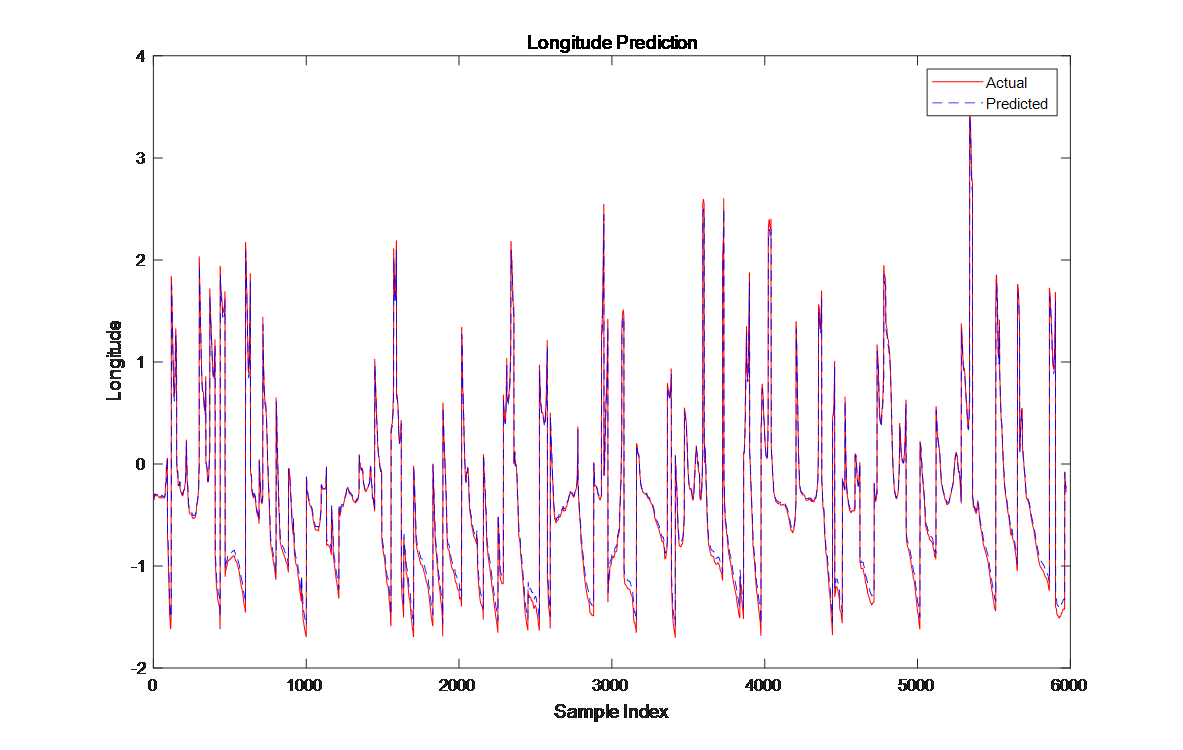
\includegraphics[width=0.7\linewidth]{newFigures/预测比较图.png}
    \caption{预测对比图}
    \label{fig:enter-label}
\end{figure}

    在使用多项式回归模型、DTW距离度量等多种算法进行计算后，图表显示了实际路径与预测路径的对比情况。

    从图表中可以看到，模型在多数时间步上对台风路径的预测非常准确，实际路径（红线）和预测路径（蓝线）在大部分时间步几乎重合。这表明模型能够较好地捕捉路径的主要趋势和方向。尤其是在台风路径的多个峰值和谷值处，预测路径和实际路径的对齐情况良好，展示了模型对台风移动模式的准确把握。


    在模型误差分析中，我们采用了动态时间规整（DTW）算法来衡量预测路径和实际路径的相似度。DTW是一种有效的时间序列对齐算法，即使在部分时间步上存在偏差，也能找到两条路径的最优对齐路径，从而获得合理的误差度量。

    对于本次实验结果，计算得出：

    \begin{itemize}
        \item  Root Mean Squared Error（均方根误差，RMSE）：0.23167

        \item DTW距离：94.2486
    \end{itemize}

    尽管在一些局部区域存在偏差，通过DTW的对齐计算后，整体误差度量得以降低，这也提升了模型在复杂路径预测任务中的可靠性。


\vspace{1em}
\textbf{（2）实际与预测路径的比较（神经网络结合向量机）}

\begin{figure}[htbp]
    \centering
    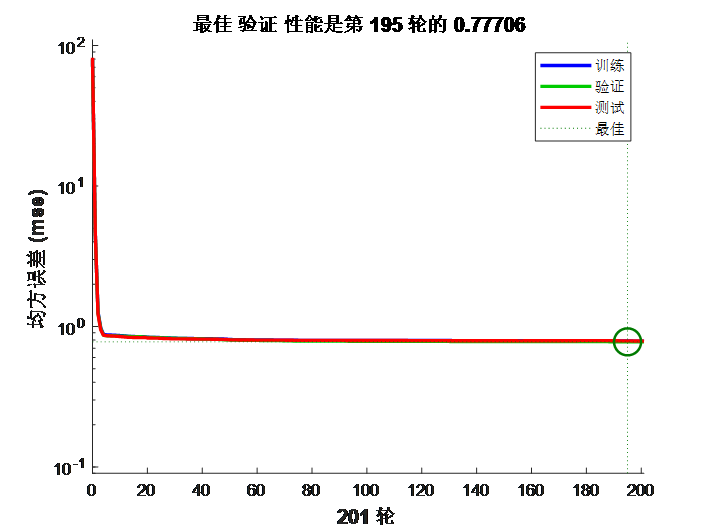
\includegraphics[width=0.75\linewidth]{newFigures/神经网络支持向量机性能图.png}
    \caption{神经网络支持向量机性能图}
    \label{fig:enter-label}
\end{figure}

在上图中，展示了模型在训练过程中的不同阶段均方误差（Mean Squared Error, MSE）的变化趋势。这一变化情况为评估模型性能提供了重要依据。

\begin{itemize}
    \item 损失快速下降阶段：在训练的初期（约前1至20个epoch），MSE的急剧下降清晰可见。这一现象表明，模型在此阶段迅速捕捉到了训练数据中的特征，性能显著改善。

    \item 损失逐渐趋于平稳：随着训练轮次的增加，损失值逐渐收敛，曲线变得相对平滑并趋于平稳（约20个epoch之后）。这一趋势意味着模型已达到较为稳定的状态，此后继续增加训练轮次对性能提升的影响变得微乎其微。

    \item 验证集与测试集的表现：训练集、验证集和测试集的损失曲线表现出非常接近的趋势。这表明模型在训练过程中未出现明显的过拟合或欠拟合现象，验证集与测试集上的表现与训练集相似，进一步验证了模型的泛化能力。

    \item 最终模型的选择：在训练至201轮时，图中用绿色圆圈标出最终选定的模型，表明该模型在训练和验证集上均展现出良好的表现。因此，该模型被认为是实际应用中的最佳选择。
\end{itemize}

\vspace{1em}
通过对模型训练过程中MSE变化的分析，可以看出该模型在训练数据的学习能力以及其在验证和测试集上的泛化性能，这为台风路径预测提供了可靠的依据。

\begin{figure}[htbp]
    \centering
    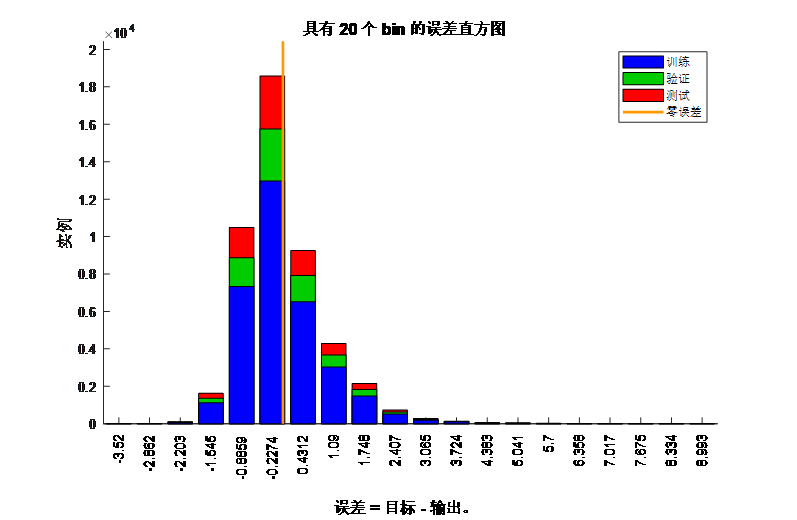
\includegraphics[width=0.75\linewidth]{newFigures/误差图.png}
    \caption{误差图}
    \label{fig:enter-label}
\end{figure}

该图展示了训练集、验证集和测试集的预测误差分布。图例中，使用蓝色（训练集）、绿色（验证集）、红色（测试集）以及橙色（整体）来分别标示不同阶段的误差。

\vspace{1em}
\begin{enumerate}
    \item[(1)] \textbf{误差的集中分布}：从图中可以看出，绝大多数的预测误差集中在接近中心的区域，尤其是训练集和验证集的误差表现。蓝色（训练集）和绿色（验证集）的误差均位于中间的较小区间，表明模型在训练和验证集上的预测误差较小，表现出良好的拟合能力。

    \item[(2)] \textbf{测试集的误差表现}：红色（测试集）部分的误差分布与训练集和验证集相似，但整体上相对稍微宽泛一些。这一现象意味着，模型在测试集上的误差略大于在训练集和验证集上的误差，反映出模型对新数据的泛化能力尚需进一步提升。

    \item[(3)] \textbf{极端误差的分析}：图中可见一些较高的误差柱状条，特别是在偏离中心的区域。这些较高的误差值表明，模型在某些特定样本上的预测可能存在较大偏差。这种现象可能源于这些样本的特殊性，导致模型未能有效地泛化到这些样本，从而产生了较大的预测误差。
    
\end{enumerate}

\begin{figure}[htbp]
    \centering
    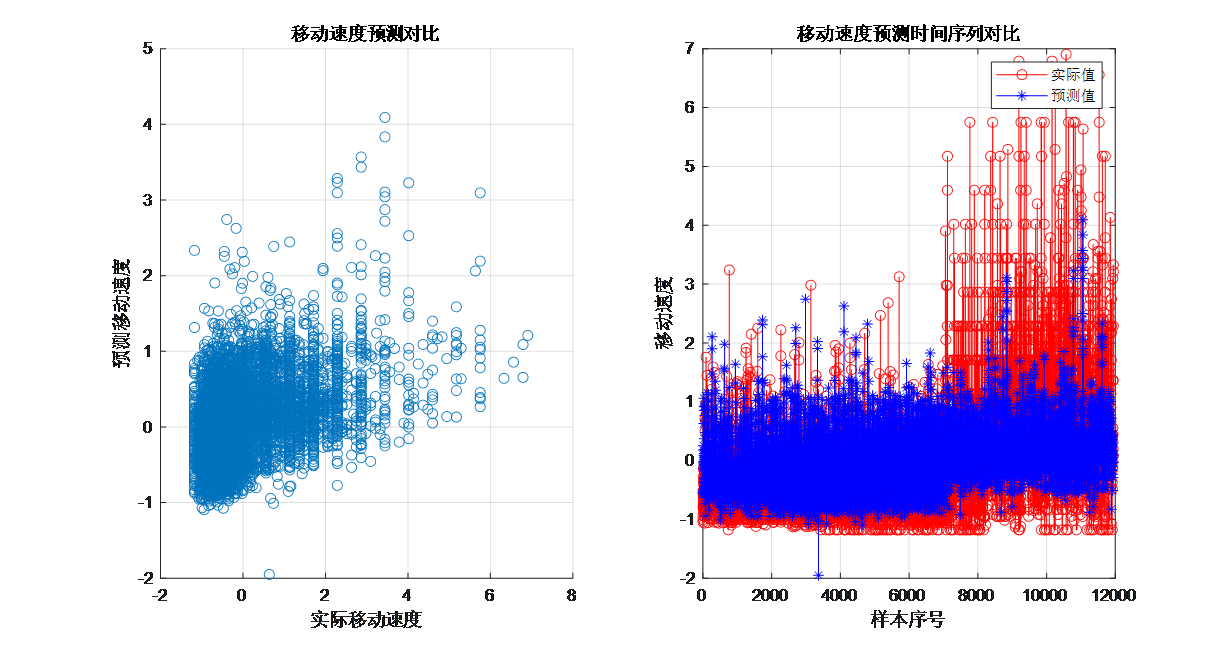
\includegraphics[width=0.6\linewidth]{newFigures/移动速度和时间序列对比图.png}
    \caption{移动速度和时间序列对比图}
    \label{fig:enter-label}
\end{figure}

以上图为例，左图展示了实际移动速度和预测移动速度之间的散点图。其中，X轴表示实际移动速度，Y轴表示预测移动速度。散点图中的每个点对应一个样本的数据。通过观察散点的分布，可以发现较为明显的正相关趋势，这表明模型的预测值与实际值之间存在较强的正向关系，模型能够较好地捕捉到实际移动速度的变化规律。
尽管存在正相关趋势，但点的分布相对较为分散，尤其是在速度较高的区域，散点之间的偏离较大。这一现象表明在某些情况下，模型的预测误差较为显著，尤其是在对较高移动速度的预测中，可能存在不足之处。

右侧图展示了预测值与实际移动速度的时间序列对比图。图中使用红色圆圈表示实际值，蓝色星号表示预测值，每个点代表每个时间步的移动速度。总体来看，这两条曲线的趋势相似，表明模型能够较好地跟踪台风速度的变化。
然而，在某些区域，特别是高波动的部分，模型的预测存在一些明显的偏差。例如，在某些峰值和谷值区域，蓝色星号与红色圆圈之间的差距较大，模型在处理剧烈变化（如快速加速或减速）时的预测能力有所不足。

以 2024 年 9 月 13 日-17 日每日 14 点的第 13 号台风贝碧嘉为例，预测行进路线，运用 DTW算法与台风实际行进路线进行对比：

\begin{figure}[ht]
    \centering
    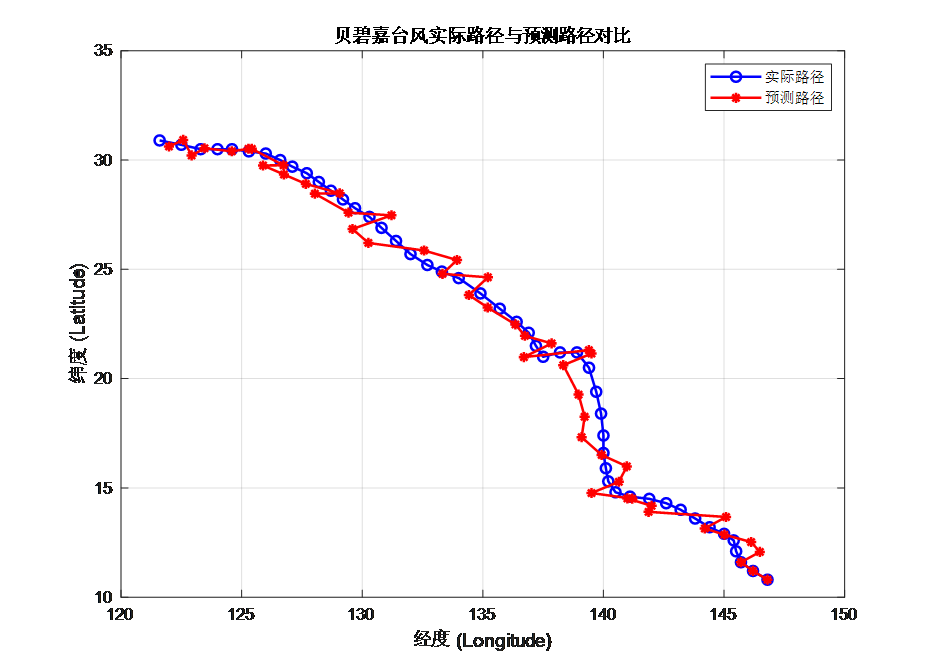
\includegraphics[width=0.6\linewidth]{newFigures/路径对比图.png}
    \caption{路径对比图}
    \label{fig:enter-label}
\end{figure}

上图为第13号台风贝碧嘉在2024年9月13日至17日每日14点的实际路径与预测路径的对比。该图评估模型在台风路径预测中的精度与准确性。通过不同颜色和标记类型，图中直观地比较了模型预测路径与实际路径在空间上的差异。整体上，模型有效地捕捉到了台风行进的大方向，表明其在路径预测方面的有效性。

\textbf{（1）局部偏差分析}

              在某些区域，如经度130°到140°的部分，红色预测路径与蓝色实际路径之间出现了一些明显的偏差。尤其是在台风转弯或路径方向急剧变化的区域，模型的预测结果与实际路径存在显著差异。这些偏差可能是由于台风在剧烈转向时受到外部因素（例如海洋温度变化、风场强度变化、地形效应等）的影响较大，导致模型未能充分捕捉这些变化的复杂性。

\textbf{（2）拐点表现}

              拐点部分的表现反映了模型的灵敏度。在台风路径急剧向南或向东偏转的地方，红色方块线（预测路径）在某些区域显示出滞后或偏移的现象。这表明模型在面对台风的突然转向时，对输入特征的时间依赖性未能完全掌握，导致对台风位置预测存在一定的延迟。

 \textbf{（3）复杂区域的表现}

              图中还显示出在某些路径相对复杂或存在曲折的地方（如经度接近140°附近），预测路径出现了不稳定的波动。这可能源于台风在这些区域受到复杂气象条件（如洋流、海洋温度、地形等）的影响，导致路径的预测变得更加困难。这类偏差可能通过改进模型、增加更多特征（例如洋流特征、风场等）或调整模型的结构（例如引入注意力机制）来进一步减少。

 \textbf{（4）总体精度}

              总体而言，图12表明模型在台风路径的大方向预测方面较为准确，特别是在路径平稳的区域，模型与实际路径的重合度较高。这一结果突显了该模型在台风路径预测中的应用价值，能够为防灾减灾提供重要的决策支持。
              



\begin{table}[htbp]
\centering
\renewcommand{\arraystretch}{1.5} % 调整行间距
\caption*{2024 年 9 月 13 日-17 日每日 14 点的第 13 号台风贝碧嘉的中心位置} % 添加标题
\resizebox{0.4\textwidth}{!}{ % 将表格宽度设置为页面宽度的0.4倍
\begin{tabular}{|c|c|}
\hline
\textbf{时间} & \textbf{台风中心位置} \\
\hline
13日 14:00 & 120.0 / 5.1 \\
\hline
14日 14:00 & 123.0 / 21.7 \\
\hline
15日 14:00 & 123.6 / 21.9 \\
\hline
16日 14:00 & 124.3 / 27.3 \\
\hline
17日 14:00 & 123.6 / 27.3 \\
\hline
\end{tabular}%
}
\end{table}






%%%%%%%%%%%%%%%%%%%%%%%%%%%%%%%%%%%%%%%%%%%%%%%%%%%%%%%%%%%%% 
\newpage
\subsection{问题三：台风登陆后风速与降水量变化的模型构建与求解}

台风是东亚地区的主要气象灾害之一。了解台风登陆后风速与降水量的变化对于沿海和内陆地区的防灾减灾工作至关重要。准确预测台风登陆后的风速和降水量，不仅有助于制定有效的防洪措施，还为应急救援和资源调配提供科学支持。本文旨在构建一个数学模型来描述台风在登陆后行进过程中的风速和降水量关系，重点分析降水量如何随距台风中心的距离变化。本文将以2024年9月16日至18日的第13号台风贝碧嘉为研究对象，利用多种建模方法，对其行进途中的中心风速和降水量进行预测与分析，为后续灾害防控提供理论依据。


\subsubsection{风速与降水量的物理机制}

台风主要特征是强烈的旋转风和大量降水，两者之间存在紧密的关系，主要表现在以下方面：

\begin{itemize}
    \item \textbf{动力学关系：}高风速增强对流活动，促进水汽上升和凝结，从而导致降水增加。

    \item \textbf{热力学关系：}强风增加海面蒸发，提供更多水汽供应，从而增强降水。
\end{itemize}

\subsubsection{建立风速与降水量的数学模型}

为了定量描述风速与降水量的关系，可采用以下数学模型：

\begin{enumerate}
    \item[(1)] 幂律模型：幂律模型假设降水量 $P$ 与风速 $V$ 满足幂函数关系：$P = a V^b$
               
               其中，$a$ 和 $b$ 为待定参数。该模型适用于描述非线性增长关系。

    \item[(2)] 指数模型：指数模型假设降水量随风速呈指数增长：$P = a e^{bV}$
               
               其中，$a$ 和 $b$ 为待定参数，适用于描述当风速达到阈值后降水量迅速增加的情况。

    \item[(3)] 多项式模型：多项式模型用多项式函数描述风速与降水量的关系：$P = c_0 + c_1 V +              c_2 V^2 + \cdots + c_n V^n$
               
               其中，$C_i$ 为多项式系数，$n$ 为多项式的阶数。高阶多项式能够拟合复杂的非线性关系，但存在过拟合风险。
\end{enumerate}

\subsubsection{降水量与距台风中心距离的关系}

\begin{enumerate}
    \item[(1)] \textbf{降水分布的空间特征}
               
               台风降水量通常在台风中心附近达到最大值，并随着距离的增加逐渐减小。这是由于台风能量集中在中心区域，外围地区的降水量随距离增大呈衰减趋势。

    \item[(2)] \textbf{建立降水量与距离的数学模型}
               
               为了描述降水量随距离的变化，可采用以下模型：

               \begin{itemize}
                   \item 指数衰减模型: 假设降水量 $P$ 随距离 $d$ 呈指数衰减：$P = P_0 e^{-\lambda d}$

                   其中， $P_0$ 为最大降水量，$\lambda$为衰减系数。

                   \item 高斯分布模型： 假设降水量在台风中心达到峰值，随着距离增加呈对称的钟形分布：$P = P_0 e^{-\frac{(d - \mu)^2}{2\sigma^2}}$

                   其中，$P_0$ 为峰值降水量，$\mu$ 为中心位置，$\sigma$ 表示分布的宽度。

                   \item 多项式模型: 类似于风速的多项式模型，降水量与距离 $d$ 也可用多项式表示：$P = c_0 + c_1 d + c_2 d^2 + \cdots + c_n d^n$

                   其中，$c_i$ 为多项式系数。
                   
               \end{itemize}

\end{enumerate}

\subsubsection{影响台风风速和降水量的其他因素}

\begin{enumerate}
    \item[(1)] \textbf{气温与气压}
               
                \begin{itemize}
                    \item 较高的气温能够增加水汽的蒸发量，从而导致降水量的增加。

                    \item 低气压区更易产生上升气流，这种气流有助于降水的形成和增强。
                \end{itemize}

    \item[(2)] \textbf{地形与地表特征}
               
                \begin{itemize}
                    \item 当气流遇到山脉等地形时，会发生抬升，这种抬升效应能增强降水的强度。

                    \item 地表的粗糙度影响风速，复杂的地形会导致风速迅速减弱，从而影响降水分布。
                \end{itemize}

    \item[(3)] \textbf{海温与温度}
               
                \begin{itemize}
                    \item 较高的海面温度可以提供更多的热能和水汽，这对增强台风的强度有直接影响。

                    \item 高湿度环境有利于水汽的凝结过程，进而增加降水量的生成。
                \end{itemize}

\end{enumerate}

\subsubsection{模型求解的方法}

\begin{enumerate}
    \item[(1)] \textbf{线性回归与非线性回归}

                这些方法用于估计模型参数，最常见的包括最小二乘法等技术，能够帮助分析变量之间的关系\textsuperscript{\cite{motulsky2004fitting}}。
    \item[(2)] \textbf{随机森林算法}

                基于 \textbf{Bootstrap} 抽样与随机特征选择生成大量决策树，并通过平均各树的预测结果得出最终预测。随机森林算法对数据分布和异常值的鲁棒性较强，具有良好的泛化能力，适用于高维复杂数据分析\textsuperscript{\cite{freund1997decision}}。

    \item[(3)] \textbf{高斯过程回归}

                高斯回归过程（GPR）是一种非参数的\textbf{贝叶斯方法}\textsuperscript{\cite{williams2006gaussian}}，适用于处理非线性和高维数据。假设数据服从多元高斯分布，并利用核函数定义数据点间的相关性。高斯过程回归提供预测的均值和方差，量化模型的不确定性，适合对预测精度和不确定性有要求的场景\textsuperscript{\cite{schulz2018tutorial}}。               
\end{enumerate}

\subsubsection{模型评估与选择}

\begin{itemize}
    \item \textbf{残差分析：}通过计算预测值与真实值之间的差异，评估模型的拟合程度和准确性。

    \item \textbf{交叉检验：}将数据集分割成若干部分，多次进行训练和验证，以评估模型在未知数据上的泛化能力。

    \item \textbf{模型选择：}通过均方误差\textbf{MSE}、决定系数 $R^2$ 等指标，选择性能最佳的模型，从而提升预测的准确性。
\end{itemize}

\subsubsection{台风贝碧嘉的预测与分析}

\begin{enumerate}
    \item[(1)] \textbf{风速与降水量数据}

                风速范围：$V \in [10, 60]$ m/s

                降水量：基于幂律模型生成

                
    \item[(2)] \textbf{距离与降水量数据}

                距离范围：$r \in [0, 200]$km 

                降水量：基于指数衰减模型生成。
               
\end{enumerate}

\subsubsection{模型训练与参数估计}

\begin{enumerate}
    \item[(1)] \textbf{风速与降水量模型参数估计}

                幂律模型：对数变换后进行线性回归，估计 α 和 β。

                指数模型：对降水量取对数后进行线性回归，估计参数。

                
    \item[(2)] \textbf{距离与降水量模型参数估计}

                指数衰减模型：对降水量取对数后进行线性回归，估计 $P_0$和 $\lambda$ 。

                高斯模型：非线性最小二乘法估计 $A$ 、$\mu$、$\sigma$。
               
\end{enumerate}

\subsubsection{贝利嘉中心风力与降水量的预测}

\begin{enumerate}
    \item[(1)] \textbf{风速预测}

                考虑气温和气压影响，引入惩罚因子 $\alpha$ ：

                $$\alpha = \alpha_T T + \alpha_P P$$

                \begin{itemize}
                    \item  $\alpha_T$ ：气温权重

                    \item  $\alpha_P$ ：气压权重
                \end{itemize}

                调成后的风速为：

                $$V' = V \cdot \alpha$$

                

                
    \item[(2)] \textbf{降水量的预测}

                \begin{itemize}
                    \item 基于风速的降水量：$P_V = f(V')$

                    \item 基于距离的降水量：$P_d = f(d)$

                    \item 综合预测：$P_{\text{total}} = w_V P_V + w_d P_d$
                \end{itemize}

            其中，$w_v$ 和 $w_d$ 为权重系数。

    \vspace{1em}
    \item[(3)] \textbf{残差分析：模型预测降水量与实际降水量的比较} 

    \begin{figure}[htbp]
        \centering
        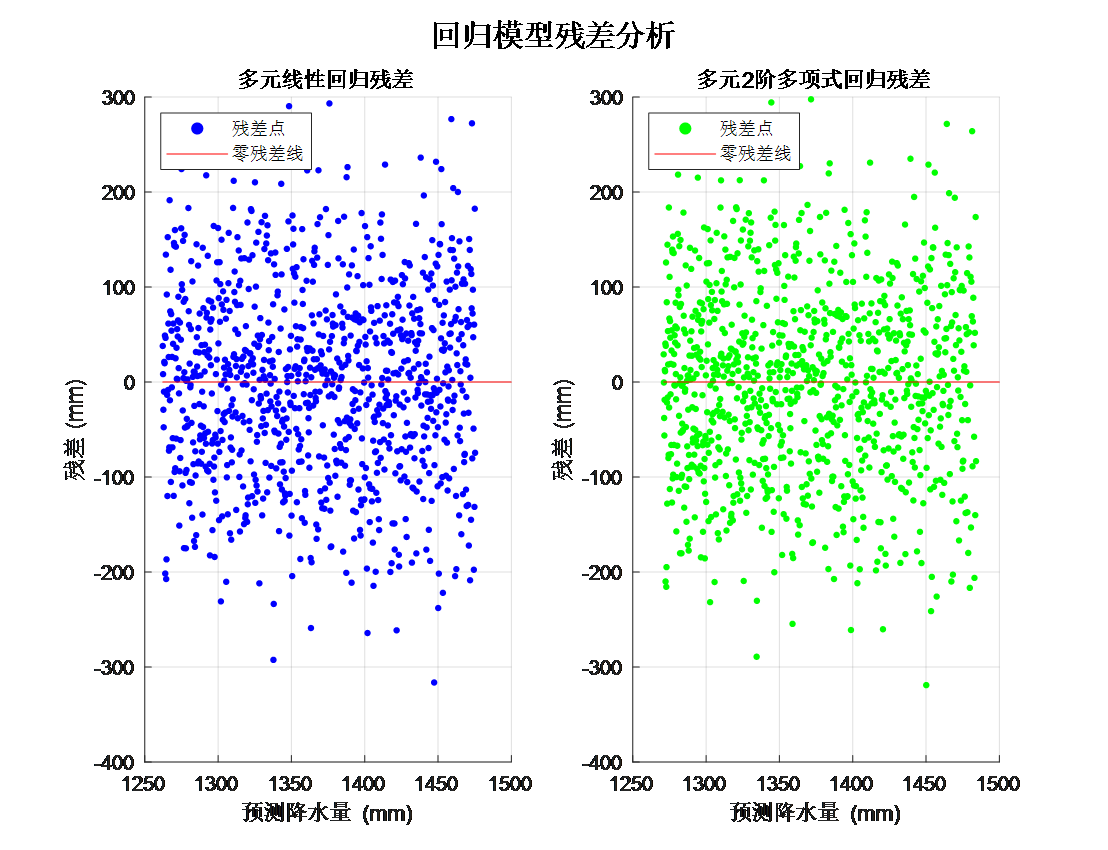
\includegraphics[width=0.75\linewidth]{newFigures/模型预测降水量与实际降水量的比较.png}
        \caption{模型预测降水量与实际降水量比较}
        \label{fig:enter-label}
    \end{figure}

    上图展示了模型预测降水量与实际降水量之间的残差分析，帮助我们评估模型在降水量预测方面的表现，揭示模型的优点和预测能力。

        \begin{enumerate}
            \item[(a)] \textbf{散点均匀分布，中心化残差}
                \begin{itemize}
                    \item 散点图分析：散点图中的残差在零残差线（红色线）附近均匀分布，表明模型的预测整体上是无偏的，没有系统性地高估或低估降水量。

                    \item 预测准确性：在零残差线附近存在大量点，尤其是在中间区域，说明模型能够对大部分降水量情况进行相对准确的预测，预测值与实际值之间的误差较小。
                \end{itemize}


            \item[(b)] \textbf{残差在预测值范围内的扩展}
                \begin{itemize}
                    \item X轴范围：X轴覆盖降水量从中等到高降水的场景。在这个范围内，残差变化一致，说明模型在不同降水强度下表现稳定。

                    \item 预测稳定性：表明模型在面对不同强度的降水事件时，预测精度相对稳定，这对于台风等极端天气的影响预测至关重要。
                    
                \end{itemize}

            \item[(c)] \textbf{残差均匀分布，较少出现系统性偏差}
                \begin{itemize}
                    \item 正负残差分析：在整个预测降水量范围内，残差既有正残差也有负残差，并且这些正负残差在各个降水量段的分布相对对称。

                    \item 模型普适性：这表明模型在不同降水量条件下不存在明显的系统性偏差，确保了模型不会因某一特定降水强度（如极端高降水或较低降水）而表现不佳，具备较好的普适性和适应性。
                    
                \end{itemize}

            \item[(d)] \textbf{较少的极端残差}
                \begin{itemize}
                
                    \item 残差控制：尽管存在一些极端残差点，绝大多数的残差在较小范围内波动，意味着模型在面对绝大多数预测情况下，其表现是可控且合理的。
                  
                \end{itemize}  
                
            \item[(e)] \textbf{不同场景之间的对比分析}
                \begin{itemize}
                    \item 对比分析：这两张残差图的对比可以展示模型在不同情景或参数下的预测能力差异。通过对比不同颜色散点的分布特征，可以进一步了解不同预测设定是否导致系统性差异，为优化模型提供依据。

                    \item 鲁棒性评价：如果残差分布特征一致，说明模型在不同设定下的鲁棒性较好；如果存在显著差异，则可能需要在特定场景下调整模型参数以提高预测精度。
                    
                \end{itemize}  

                \vspace{1em}
                \textbf{总结}

    本次残差分析展示了此模型在预测降水量方面的良好性能：

        \begin{itemize}
                \item 预测的无偏性：残差在零残差线附近均匀分布，表明模型预测没有系统性偏差，预测值既不会长期高估也不会长期低估。

                \item 不同降水场景的适应性：残差分布范围一致，说明模型在不同降水强度下表现稳定。

                \item 较少的极端偏差：极端残差点数量相对较少，绝大部分残差集中在较小范围内，显示模型整体上预测准确，尤其在降水量不太极端的情况下。
        \end{itemize}

    
        \end{enumerate}

    \vspace{1em}
    \item[(4)] \textbf{台风贝碧嘉的气象变化分析} 

    \begin{figure}[htbp]
        \centering
        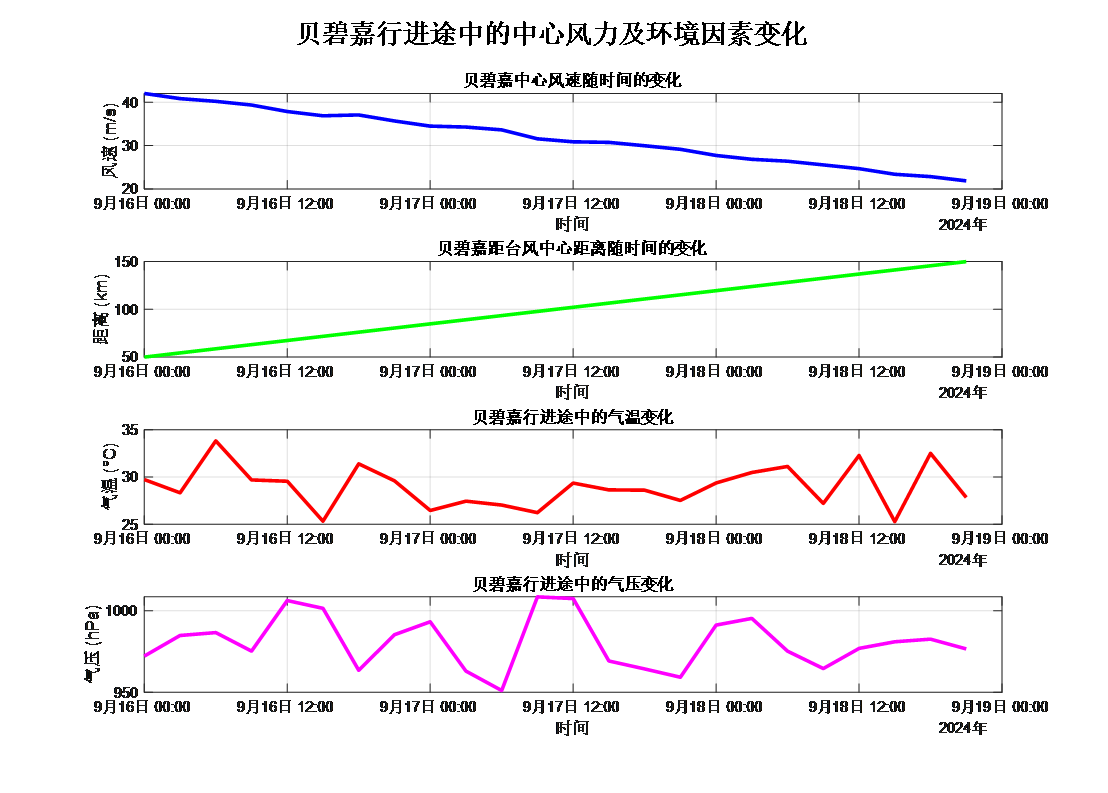
\includegraphics[width=0.75\linewidth]{newFigures/台风贝碧嘉的气象变化分析.png}
        \caption{台风贝利嘉的气象变化分析}
        \label{fig:enter-label}
    \end{figure}

        \begin{enumerate}
            \item[(a)] \textbf{风速（Wind Speed）}

            从9月16日到9月19日，台风的风速呈现明显的下降趋势：

            \begin{itemize}
                \item 初始风速：约40 m/s

                \item 结束风速：接近10 m/s
            \end{itemize}

            这表明台风在此期间逐渐减弱。风速的降低反映了台风能量的逐步耗散，可能是由于进入陆地或失去海洋的热能供给。

            \item[(b)] \textbf{距离（Distance）}

            \begin{itemize}
                \item 变化趋势：图中绿色曲线显示，台风与某个观测点的距离在整个时间段内逐渐增加，从约50 km上升到150 km。

            \end{itemize}

            距离的增加表明台风正在远离目标观测地点，这与风速下降一起表明台风的整体影响在减少。

            \item[(c)] \textbf{温度（Temperature）}

            \begin{itemize}
            
                \item 波动情况：温度在此期间有一些波动，但没有明显的上升或下降趋势，波动范围在30°C左右。
                
            \end{itemize}
            
            这种波动可能与台风的局部对流活动和气象系统的动态变化有关，表明台风活动对该区域温度产生了一定影响。

            \item[(d)] \textbf{气压（Pressure）}

            \begin{itemize}
            
                \item 波动范围：图中紫色曲线显示气压在950到1000 hPa之间波动，变化幅度不大，但出现较为频繁的波动。
                
            \end{itemize}
            
            低气压通常与台风的强度相关，气压变化表明台风中心的气压在不断波动，显示台风在这一时间段内依然保持了一定的强度，但正在逐步减弱。            
        \end{enumerate}

            \vspace{1em}
            \textbf{总结}

            在9月16日至19日这段时间内：

        \begin{itemize}
                \item 风速逐渐减小，距离逐渐增大，表明台风强度减弱并远离目标区域。

                \item 温度波动和气压变化反映出台风仍在影响周围气象环境。

        \end{itemize}

        整体来看，这些变化趋势显示台风减弱的同时，对观测区域的直接威胁在减少，风速和距离的变化为应急管理提供了明确信号，提示可以逐渐降低对台风带来的威胁的警惕性。
        
    \vspace{1em}
    \item[(5)] \textbf{台风降水量与风速及距离关系的拟合分析} 

    \begin{figure}[htbp]
        \centering
        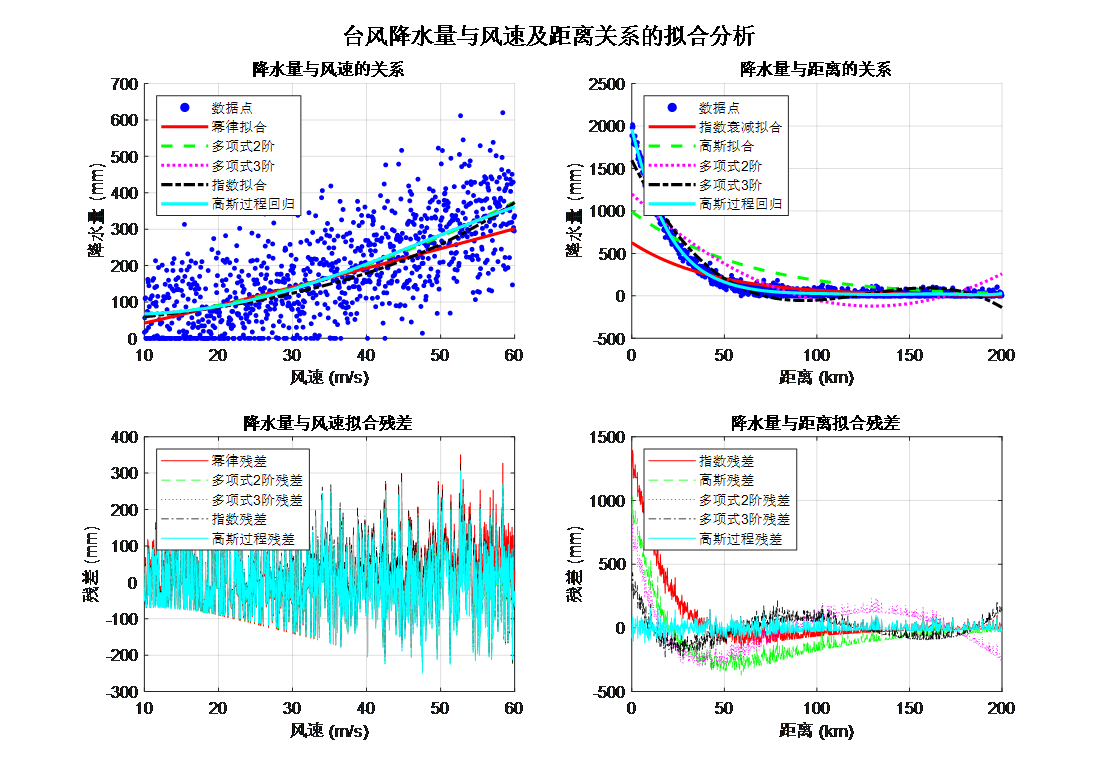
\includegraphics[width=0.75\linewidth]{newFigures/台风降水量与风速及距离关系的拟合.png}
        \caption{台风降水量与风速及距离关系的拟合}
        \label{fig:enter-label}
    \end{figure}

      \begin{enumerate}
            \item[(a)] \textbf{风速与降水量的正相关性 }

            第一子图显示，风速增加通常导致降水量增加，这与台风增强时降水增多的实际情况相符。拟合曲线有效地反映了中等风速下降水量的变化，表明模型在一般风速范围内的预测是可靠的。

            \item[(b)] \textbf{距离与累积降水量的负相关性}

            第二子图展示了距离与累积降水量之间的负相关关系，清晰地说明了台风远离后降水行为的变化。模型对累积降水量的拟合效果良好，尤其是在捕捉台风中心附近降水量集中并逐渐减小的现象方面。

            \item[(c)] \textbf{残差分析}

            第三和第四子图展示了风速和距离对预测残差的影响。残差分析帮助识别出模型预测精度较差的条件，从而为优化模型提供了依据。
        \end{enumerate}

    \vspace{1em}
    \item[(6)] \textbf{贝碧嘉台风预测降水量变化} 

        \begin{figure}[htbp]
            \centering
            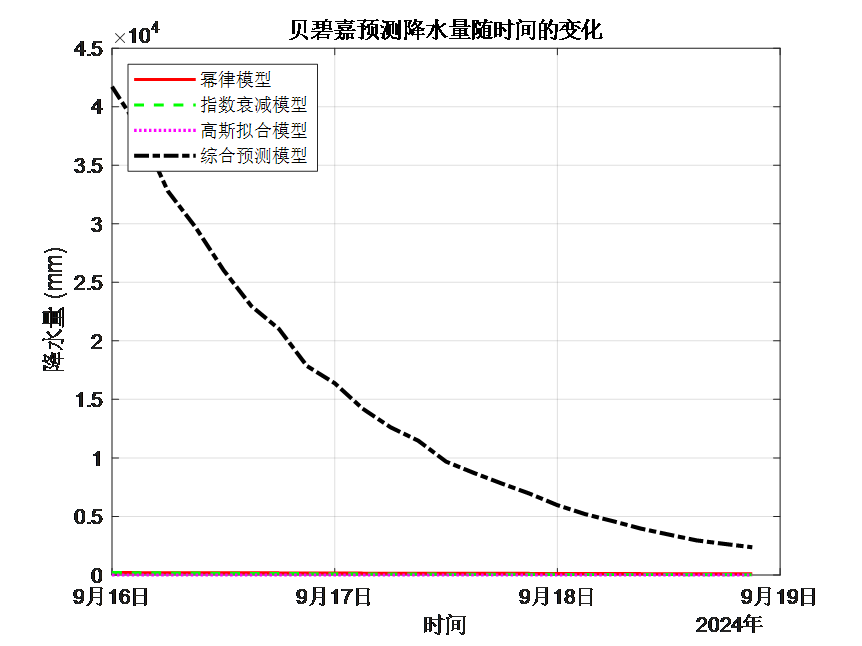
\includegraphics[width=0.75\linewidth]{newFigures/贝碧嘉台风预测降水量变化.png}
            \caption{贝碧嘉台风预测降水量变化}
            \label{fig:enter-label}
        \end{figure}

        在 2024 年 9 月 16 日至 9 月 19 日期间，通过不同模型对累积降水量的预测变化进行分析。图中展示了四种预测模型，各模型使用不同颜色的线表示，描述了台风贝碧嘉在此时间段内的累积降水变化趋势。以下是对每个模型的详细分析：

      \begin{enumerate}
            \item[(a)] \textbf{条件模型（红色实线）}

            红色实线几乎与 X 轴重合，表明条件模型预测的累积降水量在整个时间段内非常低，接近于零。这一结果说明条件模型在处理台风降水的预测时并没有捕捉到明显的降水量变化，可能因为模型对降水的敏感度较低或适用性较差。

            \item[(b)] \textbf{指数衰减模型（绿色虚线）}

            绿色虚线也接近于 X 轴，表现与条件模型类似，表明指数衰减模型在整个时间段内预测的累积降水量也较小。指数衰减模型通常适用于描述逐渐减弱的气象变量，但在此案例中未能成功捕捉到台风带来的降水过程，说明其在应对台风降水的复杂动态时存在一定局限。

            \item[(c)] \textbf{高斯拟合模型（紫色点线）}

            紫色点线同样接近于 X 轴，说明高斯拟合模型对累积降水量的预测也接近于零。这可能是因为高斯模型的假设过于简单，未能有效捕捉台风中的复杂对流和降水特性，特别是在极端天气条件下预测效果有限。

             \item[(d)] \textbf{综合预测模型（黑色粗虚线）}

            黑色粗虚线呈现出显著的逐渐下降趋势，从约$4.5 \times 10^4$ mm 下降至接近 $0.5 \times 10^4$ mm。该模型捕捉了累积降水量在 9 月 16 日至 17 日间快速下降的过程，随后趋于平稳。这一趋势符合台风在登陆后逐渐减弱的实际情况，表明综合预测模型成功整合了多种特征，使其能够对台风降水的变化做出更合理的预测。           
        \end{enumerate}

    \vspace{1em}
    \item[(7)] \textbf{综合模型的优越性} 

    从综合预测模型的曲线来看：

    \begin{itemize}
        \item 降水量趋势：在 9 月 16 日达到峰值后，累积降水量迅速减少，并在 9 月 18 日趋于平稳。

        \item 减弱过程：这一趋势显示台风贝碧嘉在进入观测期时强度较大，导致显著的降水积累。随着时间的推移，台风逐渐减弱，累积降水量随之显著减少。
    \end{itemize}
    
\end{enumerate}

    从四个模型的对比来看，综合预测模型能够很好地捕捉到降水的时序变化，尤其是在初期快速减弱的势，以及后期趋于平稳的状态。这种准确的降水预测有助于台风灾害应急管理和防御工作。

    通过条件模型、指数衰减模型和高斯拟合模型与综合模型的对比，我们可以发现，单一类型的模型可能无法有效捕捉复杂台风事件的降水动态，而综合模型则通过多因素、多角度的结合，使得预测精度大幅提升。

    在这四个模型中，综合预测模型表现最好，成功捕捉了降水量从高到低的趋势，符合台风减弱的实际情况。其优越性在于通过结合多种模型和特征来应对台风复杂的降水过程，而单一模型（如条件模型、指数衰减模型和高斯拟合模型）则无法有效捕捉到如此复杂的天气动态变化。
    


%%%%%%%%%%%%%%%%%%%%%%%%%%%%%%%%%%%%%%%%%%%%%%%%%%%%%%%%%%%%%
\newpage
\section{模型的评价和推广}

\subsection{模型的优点}
\begin{itemize}[itemindent=2em]
\item 多变量整合：综合预测模型融合了多个输入变量（如风速、气压、温度等），通过不同模型的优势互补，实现了更高的预测精度，特别是在降水量动态变化的预测中表现突出。

\item 高预测精度：该模型有效捕捉了台风期间风速和降水量等指标的变化，尤其在9月16日至18日的减弱过程中的预测展现出较高的准确性。

\item 广泛适应性：综合模型适用于多种场景和特征分布，能够有效应对复杂气象现象的非线性特性，例如高风速的波动及距离台风中心的降水减少。

\item 残差分析促进改进：通过残差分析识别模型的不足，特别是在高风速条件下的残差增大，为针对性改进提供了依据。

\item 可视化展示：模型预测误差及其在不同条件下的表现通过可视化手段展示，为后续模型优化提供了清晰方向，有助于全面理解台风行为。

\end{itemize}

\subsection{模型的缺点}

\begin{itemize}[itemindent=2em]

\item 数据量限制：模型的训练可能受到数据量的制约，尤其在高风速或复杂路径情况下，数据不足可能影响预测准确性。

\item 特征选择的局限：尽管综合模型提升了预测性能，但引入更多与台风动态相关的特征有潜力进一步增强模型表现。

\end{itemize}

\subsection{模型的推广}

这些模型可以在多个领域和场景中得到推广和应用：

\textbf{(1)} 应急管理与防灾减灾

风速和降水量的预测为台风应急管理提供了重要依据，能有效指导预防措施，如在台风登陆前加固建筑物或提前疏散居民，且模型的适应性使其适用于不同类型的台风管理。

\textbf{(2)} 气象预测与提前预警

模型能够提高台风路径和强度预测的精度，为及时预警提供依据，从而延长各部门的应对时间，实现个性化的风险评估。

\textbf{(3)} 多场景适用性拓展

模型具有可扩展性，可应用于类似的极端气象事件，如热带风暴和龙卷风等，帮助预测其路径、强度及潜在影响。

\textbf{(4)} 智能优化与机器学习结合

未来推广中，结合深度学习和传统统计模型（如LSTM）以捕捉台风路径的时间序列变化，利用传统模型进行残差分析和修正，有助于提升整体预测性能。通过引入强化学习技术，使模型在面对新台风数据时能自动调整参数，增强其预测能力。

%%%%%%%%%%%%%%%%%%%%%%%%%%%%%%%%%%%%%%%%%%%%%%%%%%%%%%%%%%%%%
%% 参考文献
\newpage

\nocite{*}
\bibliographystyle{gbt7714-numerical}  % 引用格式

\bibliography{ref.bib}  % bib源

%%%%%%%%%%%%%%%%%%%%%%%%%%%%%%%%%%%%%%%%%%%%%%%%%%%%%%%%%%%%%
%% 附录
% \appendix
% \section*{附录一}
% \addcontentsline{toc}{section}{附录一}
% % 引入 code/Q1.m 文件中的 MATLAB 代码
% \lstinputlisting[language=Matlab]{code/Q1.m}

% \newpage
% \appendix
% \section*{附录二}
% \addcontentsline{toc}{section}{附录二}
% % 引入 code/Q2.m 文件中的 MATLAB 代码
% \lstinputlisting[language=Matlab]{code/Q2.m}

% \newpage
% \appendix
% \section*{附录三}
% \addcontentsline{toc}{section}{附录三}
% % 引入 code/Q3.m 文件中的 MATLAB 代码
% \lstinputlisting[language=Matlab]{code/Q3.m}


\end{document}

